\documentclass[a4paper,14pt]{extarticle}

% -------------------- Кодировка и языки --------------------
\usepackage[russian]{babel}

% -------------------- Шрифты --------------------
\usepackage{fontspec}
\setmainfont{Times New Roman}

% -------------------- Геометрия страницы --------------------
\usepackage[
    left=3cm,
    right=1cm,
    top=2cm,
    bottom=2cm
]{geometry}

\setlength{\footskip}{62pt}

% -------------------- Межстрочный интервал --------------------
\usepackage{setspace}
\onehalfspacing

% -------------------- Абзацный отступ --------------------
\usepackage{indentfirst}
\setlength{\parindent}{1.25cm}

% -------------------- Работа с графикой и таблицами --------------------
\usepackage{graphicx}
\usepackage{float}
\usepackage{caption}
\usepackage{booktabs}
\usepackage{longtable}
\usepackage{array}

% Подписи рисунков и таблиц
\addto\captionsrussian{%
    \renewcommand{\figurename}{Рисунок}
    \renewcommand{\tablename}{Таблица}
}
\captionsetup{
    labelsep=endash,
    justification=centering
}

% -------------------- Гиперссылки --------------------
\usepackage[hidelinks]{hyperref}

% -------------------- Листинги кода --------------------
\usepackage{listings}
\usepackage{xcolor}

\definecolor{codebg}{RGB}{245,245,245}
\lstset{
    basicstyle=\ttfamily\small,
    backgroundcolor=\color{codebg},
    frame=single,
    breaklines=true,
    columns=fullflexible,
    keepspaces=true,
    showstringspaces=false
}

% -------------------- Заголовки --------------------
\usepackage{titlesec}

\titleformat{\section}
  {\normalfont\bfseries\centering}
  {\thesection}
  {1em}
  {}

\titleformat{\subsection}
  {\normalfont\bfseries\centering}
  {\thesubsection}
  {1em}
  {}

\titleformat{\subsubsection}
  {\normalfont\bfseries\centering}
  {\thesubsubsection}
  {1em}
  {}

% -------------------- Нумерация страниц --------------------
\usepackage{fancyhdr}
\pagestyle{fancy}
\fancyhf{}
\fancyhead[C]{\thepage}
\renewcommand{\headrulewidth}{0pt}
\setlength{\headheight}{17pt} % Исправляет предупреждение о headheight

% -------------------- Название оглавления --------------------
\renewcommand{\contentsname}{ОГЛАВЛЕНИЕ}

\begin{document}

% Тут содержимое документа


% ============================================================
% ТИТУЛЬНЫЙ ЛИСТ
% ============================================================
\thispagestyle{empty}
\begin{titlepage}
    \thispagestyle{empty}

    \begin{center}
        \textbf{} \\[0.5cm]
        \textbf{} \\[0.5cm]
        \textbf{}
    \end{center}

    \vspace{3cm}

    \begin{center}
        \textbf{\Large Техническое описание решения} \\[0.5cm]
        \textbf{\large по направлению} \\[0.5cm]
        \textbf{\Large «Системный анализ и суперкомпьютерное моделирование »}
    \end{center}

    \vspace{4cm}

    \begin{flushright}
        Самойлов Михаил Андреевич \\ 
        Магелатова Валерия Сергеевна \\ 
        Чванов Александр Вячеславович
    \end{flushright}

    \vfill

    

    \begin{center}
        Москва \\
        2026
    \end{center}

    
\end{titlepage}

% Начиная со 2 страницы показываем номер
\setcounter{page}{1}

% ============================================================
% ОГЛАВЛЕНИЕ
% ============================================================
\tableofcontents
\newpage

% ============================================================
% ДАЛЬШЕ ПОЙДЕТ ТЕКСТ РАБОТЫ
% ============================================================

\section{Введение}
Система доменных имён DNS является одной из ключевых составляющих современной сетевой инфраструктуры. От корректности и скорости её работы напрямую зависят доступность веб-ресурсов, прикладных сервисов и различных распределённых систем. Одним из основных механизмов повышения производительности DNS-резолверов является кэширование ответов. В стандартной модели время хранения записей определяется полем TTL, которое задаётся авторитетным сервером доменной зоны. Однако в ряде практических сценариев возникает необходимость управлять временем хранения ответов независимо от исходного TTL: например, для повышения устойчивости инфраструктуры, снижения числа внешних обращений, организации локального переопределения ответов или построения долговременного внешнего кэша.

Актуальность работы обусловлена необходимостью исследования механизмов кэширования DNS-ответов на время, отличное от исходного TTL, а также проверкой практической реализуемости такого подхода на базе современного DNS-резолвера.

Целью работы является исследование и реализация механизмов кэширования DNS-ответов на время, отличное от TTL, с использованием встроенных средств резолвера Unbound и внешнего хранилища Redis.

Для достижения поставленной цели были сформулированы следующие задачи:
\begin{enumerate}
    \item исследовать стандартные средства кэширования резолвера Unbound;
    \item проверить работу базового кэширования, механизма prefetch и параметров принудительного изменения времени хранения записей;
    \item продемонстрировать ограничения встроенного кэша и возможность вытеснения записей до истечения принудительно установленного времени хранения;
    \item реализовать внешний кэш DNS-ответов на базе Redis;
    \item обеспечить формирование DNS-ответов непосредственно из внешней базы данных;
    \item показать возможность локального переопределения DNSSEC-подписанной зоны на уровне собственного резолвера.
\end{enumerate}

Объектом исследования является DNS-резолвер Unbound. Предметом исследования являются механизмы кэширования DNS-ответов, способы принудительного увеличения времени хранения записей и интеграция внешнего хранилища ответов.

Практическая значимость работы состоит в разработке и экспериментальной проверке подхода, позволяющего расширить стандартные возможности DNS-резолвера и организовать долговременное управляемое кэширование ответов.
\section{Общее описание архитектуры}
Для проведения экспериментов был подготовлен локальный стенд на базе Docker Compose, включающий контейнер с DNS-резолвером Unbound и контейнер с Redis. Резолвер Unbound использовался как основной компонент обработки DNS-запросов, Redis --- как внешняя база данных для долговременного хранения DNS-ответов. Дополнительно в стенде использовались инструменты сетевой диагностики, в частности \texttt{dig} и \texttt{tcpdump}.

Запуск окружения выполнялся следующими командами:

\begin{lstlisting}
docker compose up -d --build unbound
docker compose up -d redis
docker compose ps
\end{lstlisting}

При необходимости пересборки и перезапуска контейнеров использовались команды:

\begin{lstlisting}
docker compose up -d --build unbound
docker compose up -d --build redis
\end{lstlisting}

Для очистки внешнего кэша Redis применялась команда:

\begin{lstlisting}
docker compose exec redis redis-cli FLUSHALL
\end{lstlisting}

Логика обработки DNS-запроса в исследуемом стенде состояла в следующем. Клиент отправляет запрос в Unbound. Далее резолвер последовательно проверяет наличие локального переопределения зоны, наличие готового ответа во внешнем кэше Redis и, при отсутствии совпадения, выполняет стандартное рекурсивное разрешение через корневые, TLD- и авторитетные DNS-серверы. После получения ответа он может быть сохранён во внешний кэш и использован при последующих обращениях.

\begin{figure}[H]
    \centering
    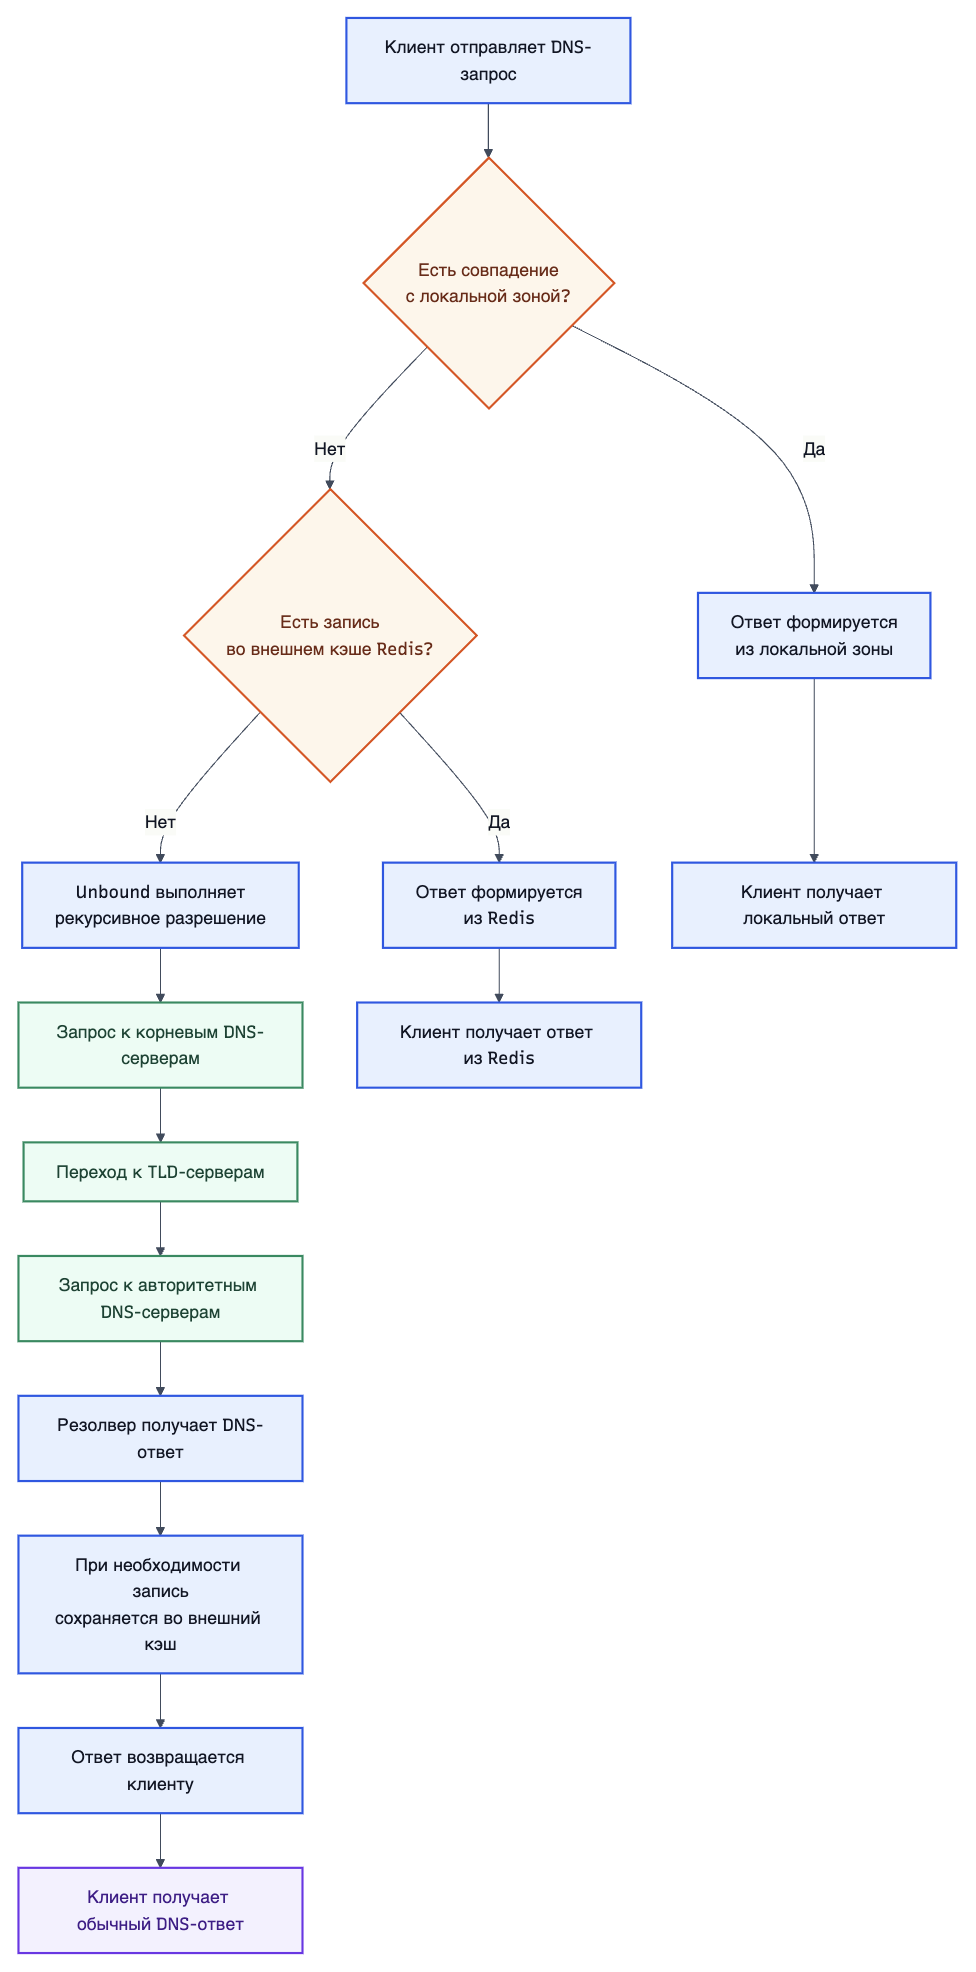
\includegraphics[width=0.65\textwidth]{assets/architecture.png}
    \caption{Общая схема обработки DNS-запроса в исследуемом стенде}
\end{figure}


\subsection{Описание стенда}
\subsection{Схема обработки DNS-запроса}
\subsection{Используемые инструменты}

\section{Методика кэширование ответов на время отличное от времени TTL}

\subsection{Методика определения источника DNS-ответа}
Для определения источника DNS-ответа использовались три независимых признака.

Во-первых, анализировалось время ответа на повторный запрос. Если повторный ответ возвращался существенно быстрее первого, это указывало на использование кэша.

Во-вторых, анализировалось изменение TTL. Если при повторном запросе значение TTL уменьшалось на интервал, близкий ко времени ожидания между запросами, это свидетельствовало о выдаче данных из кэша резолвера.

В-третьих, использовался анализ сетевого трафика с помощью \texttt{tcpdump}. Для этого во втором терминале запускалось наблюдение за DNS-трафиком внутри контейнера Unbound:

\begin{lstlisting}
docker exec -it dns-unbound tcpdump -tttt -n -i any '(udp port 53 or tcp port 53)'
\end{lstlisting}

Интерпретация результатов выполнялась следующим образом:
\begin{itemize}
    \item если в трассировке наблюдались исходящие DNS-запросы Unbound во внешнюю сеть, фиксировался случай \textit{cache miss};
    \item если наблюдался только входящий клиентский запрос и немедленный исходящий ответ клиенту без внешних обращений, фиксировался случай \textit{cache hit};
    \item если ответ клиенту выдавался быстро, но после этого резолвер выполнял внешние DNS-запросы, это указывало на срабатывание механизма \textit{prefetch}.
\end{itemize}

Таким образом, источник DNS-ответа определялся не по одному косвенному признаку, а по совокупности временных характеристик, изменения TTL и сетевой трассировки.

\subsection{(1.1А) Проверка базового кэширования на примере \texttt{yandex.ru}}
Целью первого эксперимента являлась проверка того, что резолвер Unbound сохраняет DNS-ответ во встроенном кэше и использует его при повторном обращении до истечения TTL.

Для эксперимента был выбран домен \texttt{yandex.ru} и выполнены два запроса с интервалом 5 секунд:

\begin{lstlisting}
dig @127.0.0.1 -p 2053 yandex.ru A
sleep 5
dig @127.0.0.1 -p 2053 yandex.ru A
\end{lstlisting}

\begin{figure}[H]
    \centering
    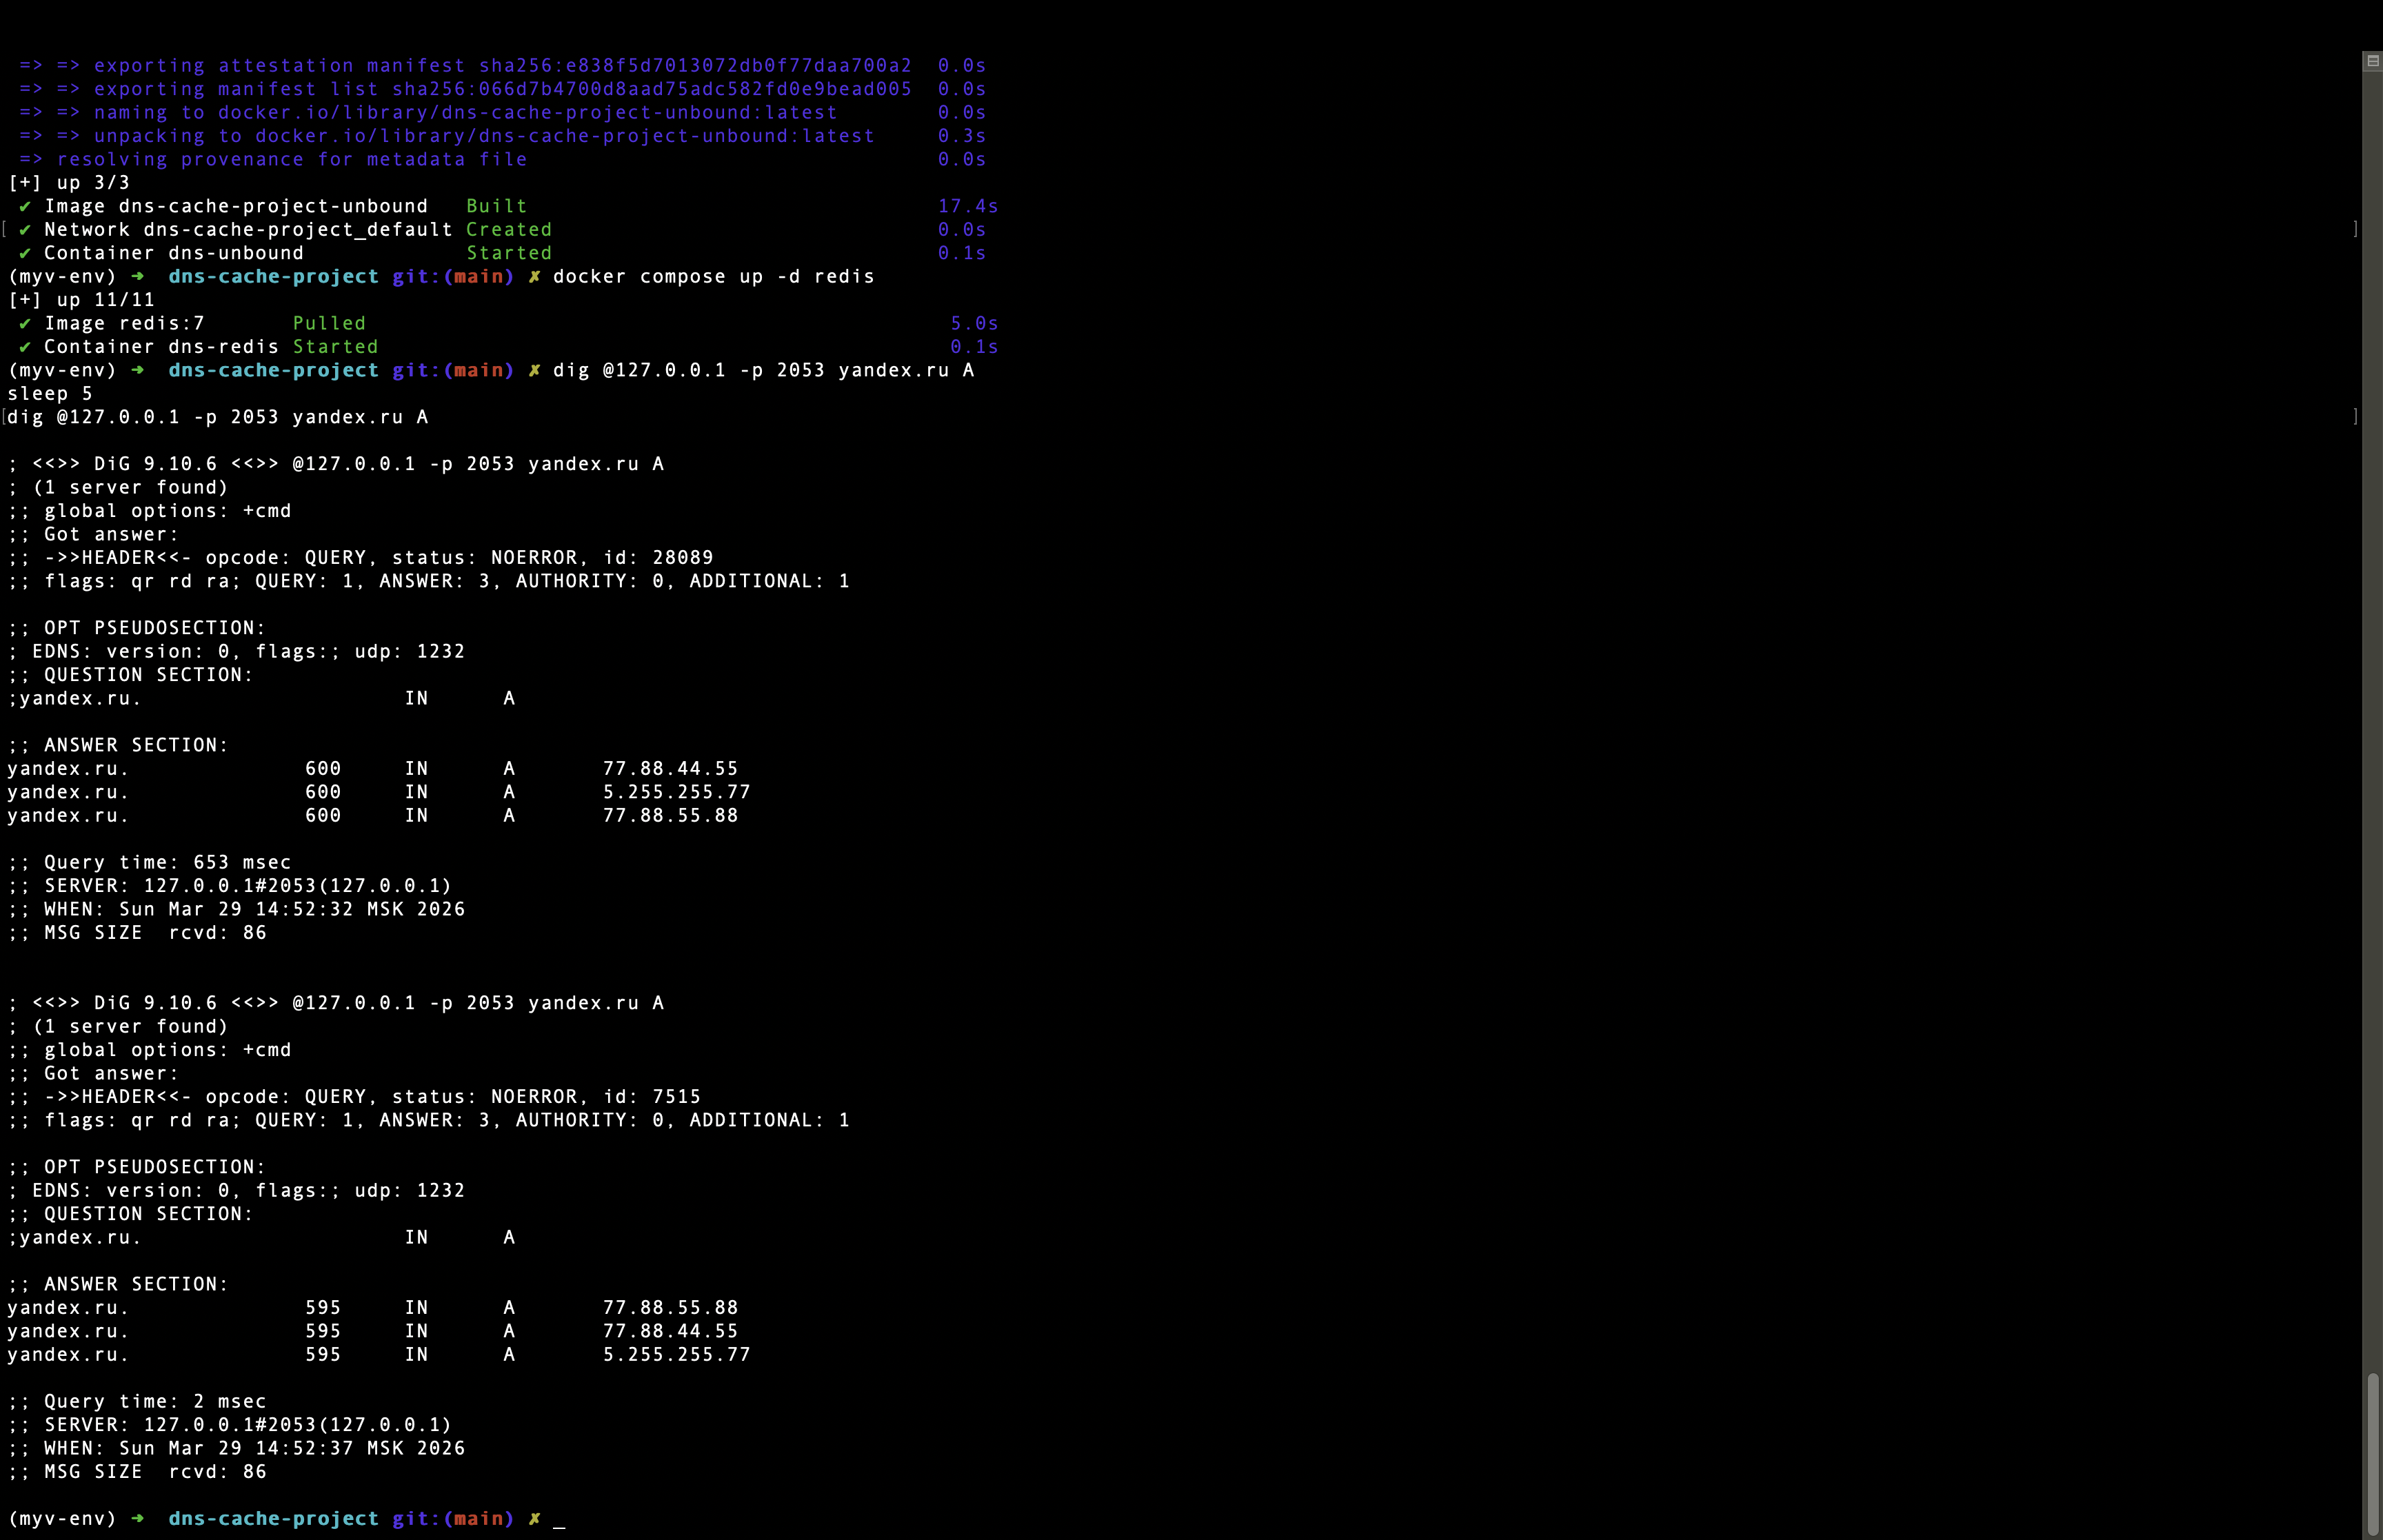
\includegraphics[width=0.95\textwidth]{assets/terminal_screenshot_1.png}
    \caption{Результаты первичного и повторного DNS-запросов к домену \texttt{yandex.ru}}
\end{figure}

По результатам эксперимента были получены следующие наблюдения:
\begin{itemize}
    \item время ответа уменьшилось с 653 мс до 2 мс;
    \item значение TTL изменилось с 600 до 595 секунд;
    \item уменьшение TTL соответствовало интервалу ожидания между запросами.
\end{itemize}

Фрагмент ответа имел следующий вид:

\begin{lstlisting}
Query time: 653 msec -> Query time: 2 msec

yandex.ru.      600 IN A 77.88.44.55
yandex.ru.      600 IN A 5.255.255.77
yandex.ru.      600 IN A 77.88.55.88

yandex.ru.      595 IN A 77.88.55.88
yandex.ru.      595 IN A 77.88.44.55
yandex.ru.      595 IN A 5.255.255.77
\end{lstlisting}

Для дополнительного подтверждения был выполнен анализ сетевого трафика.

\begin{figure}[H]
    \centering
    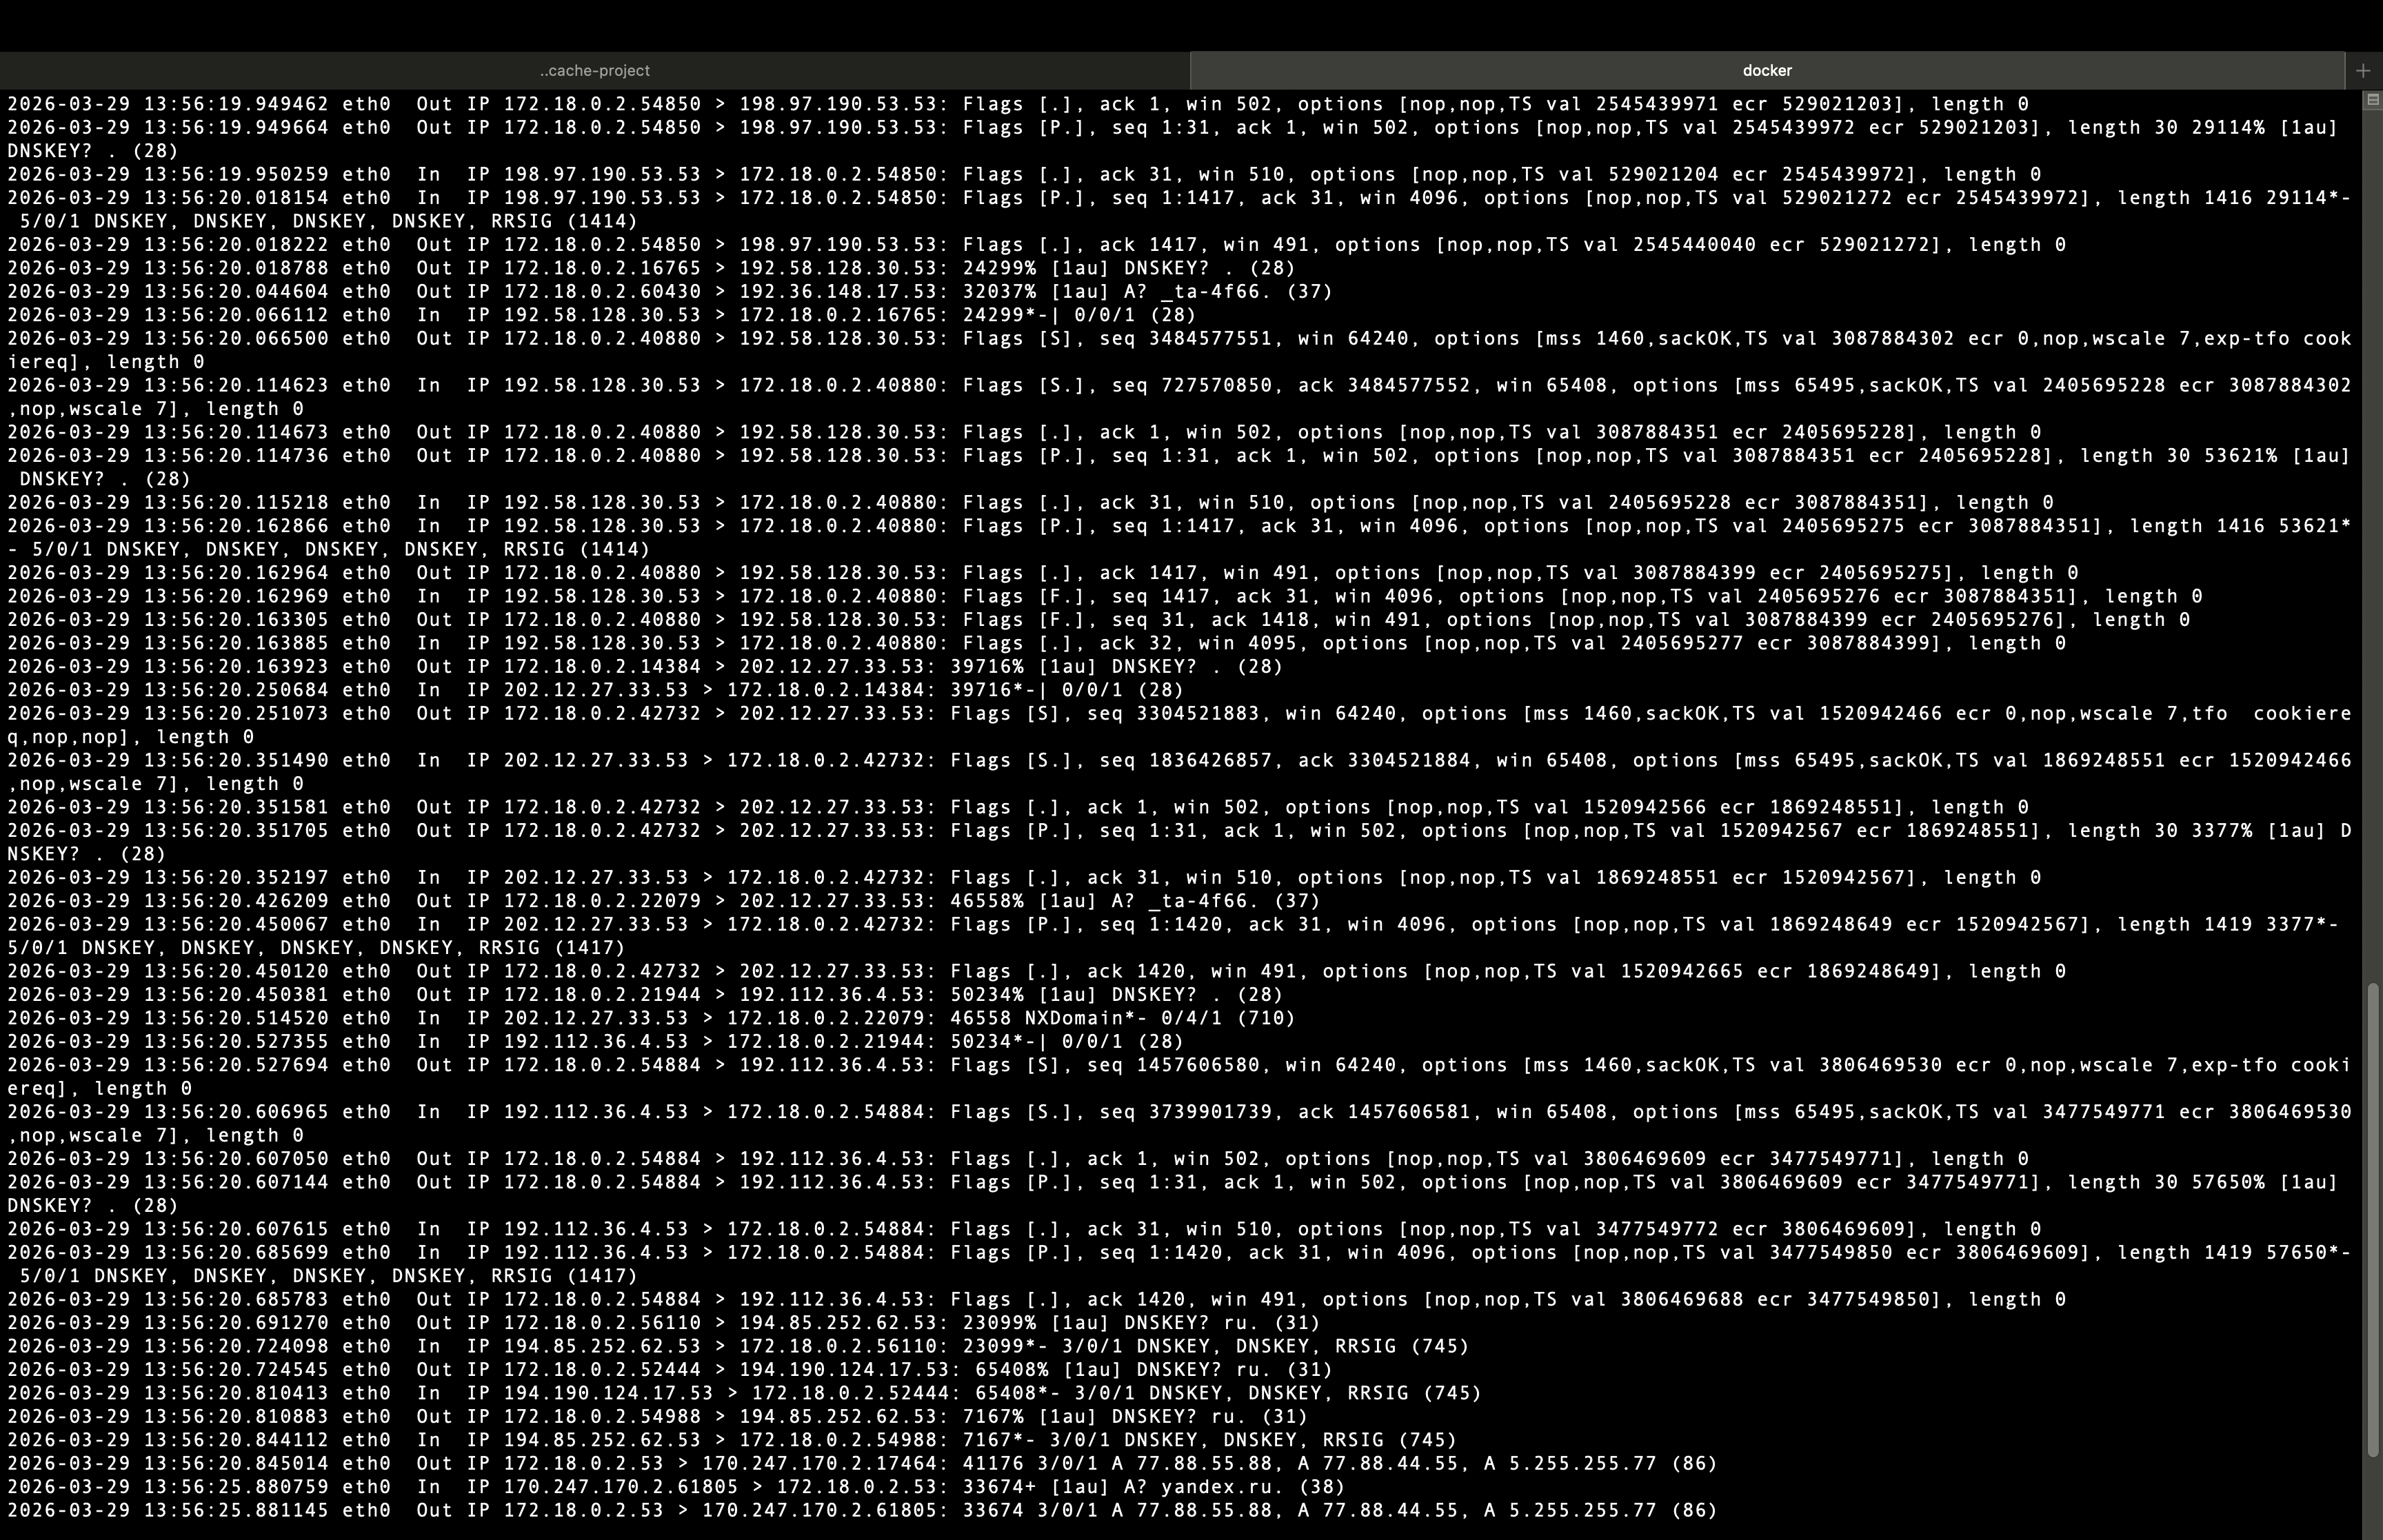
\includegraphics[width=0.95\textwidth]{assets/terminal_screenshot_1_tcpdump.png}
    \caption{Анализ DNS-трафика при повторном обращении к \texttt{yandex.ru}}
\end{figure}

При первом запросе 
\begin{lstlisting}
2026-03-29 13:56:20.845014 eth0  Out IP 172.18.0.2.53 > 170.247.170.2.17464: 41176 3/0/1 A 77.88.55.88, A 77.88.44.55, A 5.255.255.77 (86)
\end{lstlisting}

При втором запросе 
\begin{lstlisting}
2026-03-29 13:56:25.880759 eth0  In  IP 170.247.170.2.61805 > 172.18.0.2.53: 33674+ [1au] A? yandex.ru. (38)
2026-03-29 13:56:25.881145 eth0  Out IP 172.18.0.2.53 > 170.247.170.2.61805: 33674 3/0/1 A 77.88.55.88, A 77.88.44.55, A 5.255.255.77 (86)
\end{lstlisting}

При первом запросе в трассировке присутствовало внешнее обращение резолвера, а при втором запросе наблюдалась только пара \textit{входящий запрос клиента --- исходящий ответ клиенту} без нового внешнего DNS-запроса для \texttt{yandex.ru}. Это подтверждает, что повторный ответ был выдан из встроенного кэша Unbound.

Следовательно, стандартный механизм кэширования Unbound функционирует корректно: ответ сохраняется во встроенном кэше и используется повторно до истечения TTL.

\subsection{Проверка механизма prefetch}
Следующим этапом была проверка механизма \textit{prefetch}, который позволяет обновлять записи в кэше до их полного истечения. В исследуемой конфигурации Unbound функция была включена директивой:

\begin{lstlisting}
prefetch: yes
\end{lstlisting}

Механизм \textit{prefetch} работает следующим образом: если в кэше уже присутствует запись с TTL, близким к исчерпанию, и поступает новый запрос к этой записи, резолвер немедленно отдаёт клиенту имеющийся ответ, а затем в фоновом режиме инициирует обновление данных.

Для проверки использовался домен \texttt{yandex.ru}. После предварительного прогрева кэша выполнялся запрос в момент, когда оставшийся TTL был близок к завершению:

\begin{lstlisting}
dig @127.0.0.1 -p 2053 yandex.ru A
sleep 530
dig @127.0.0.1 -p 2053 yandex.ru A
\end{lstlisting}

\begin{figure}[H]
    \centering
    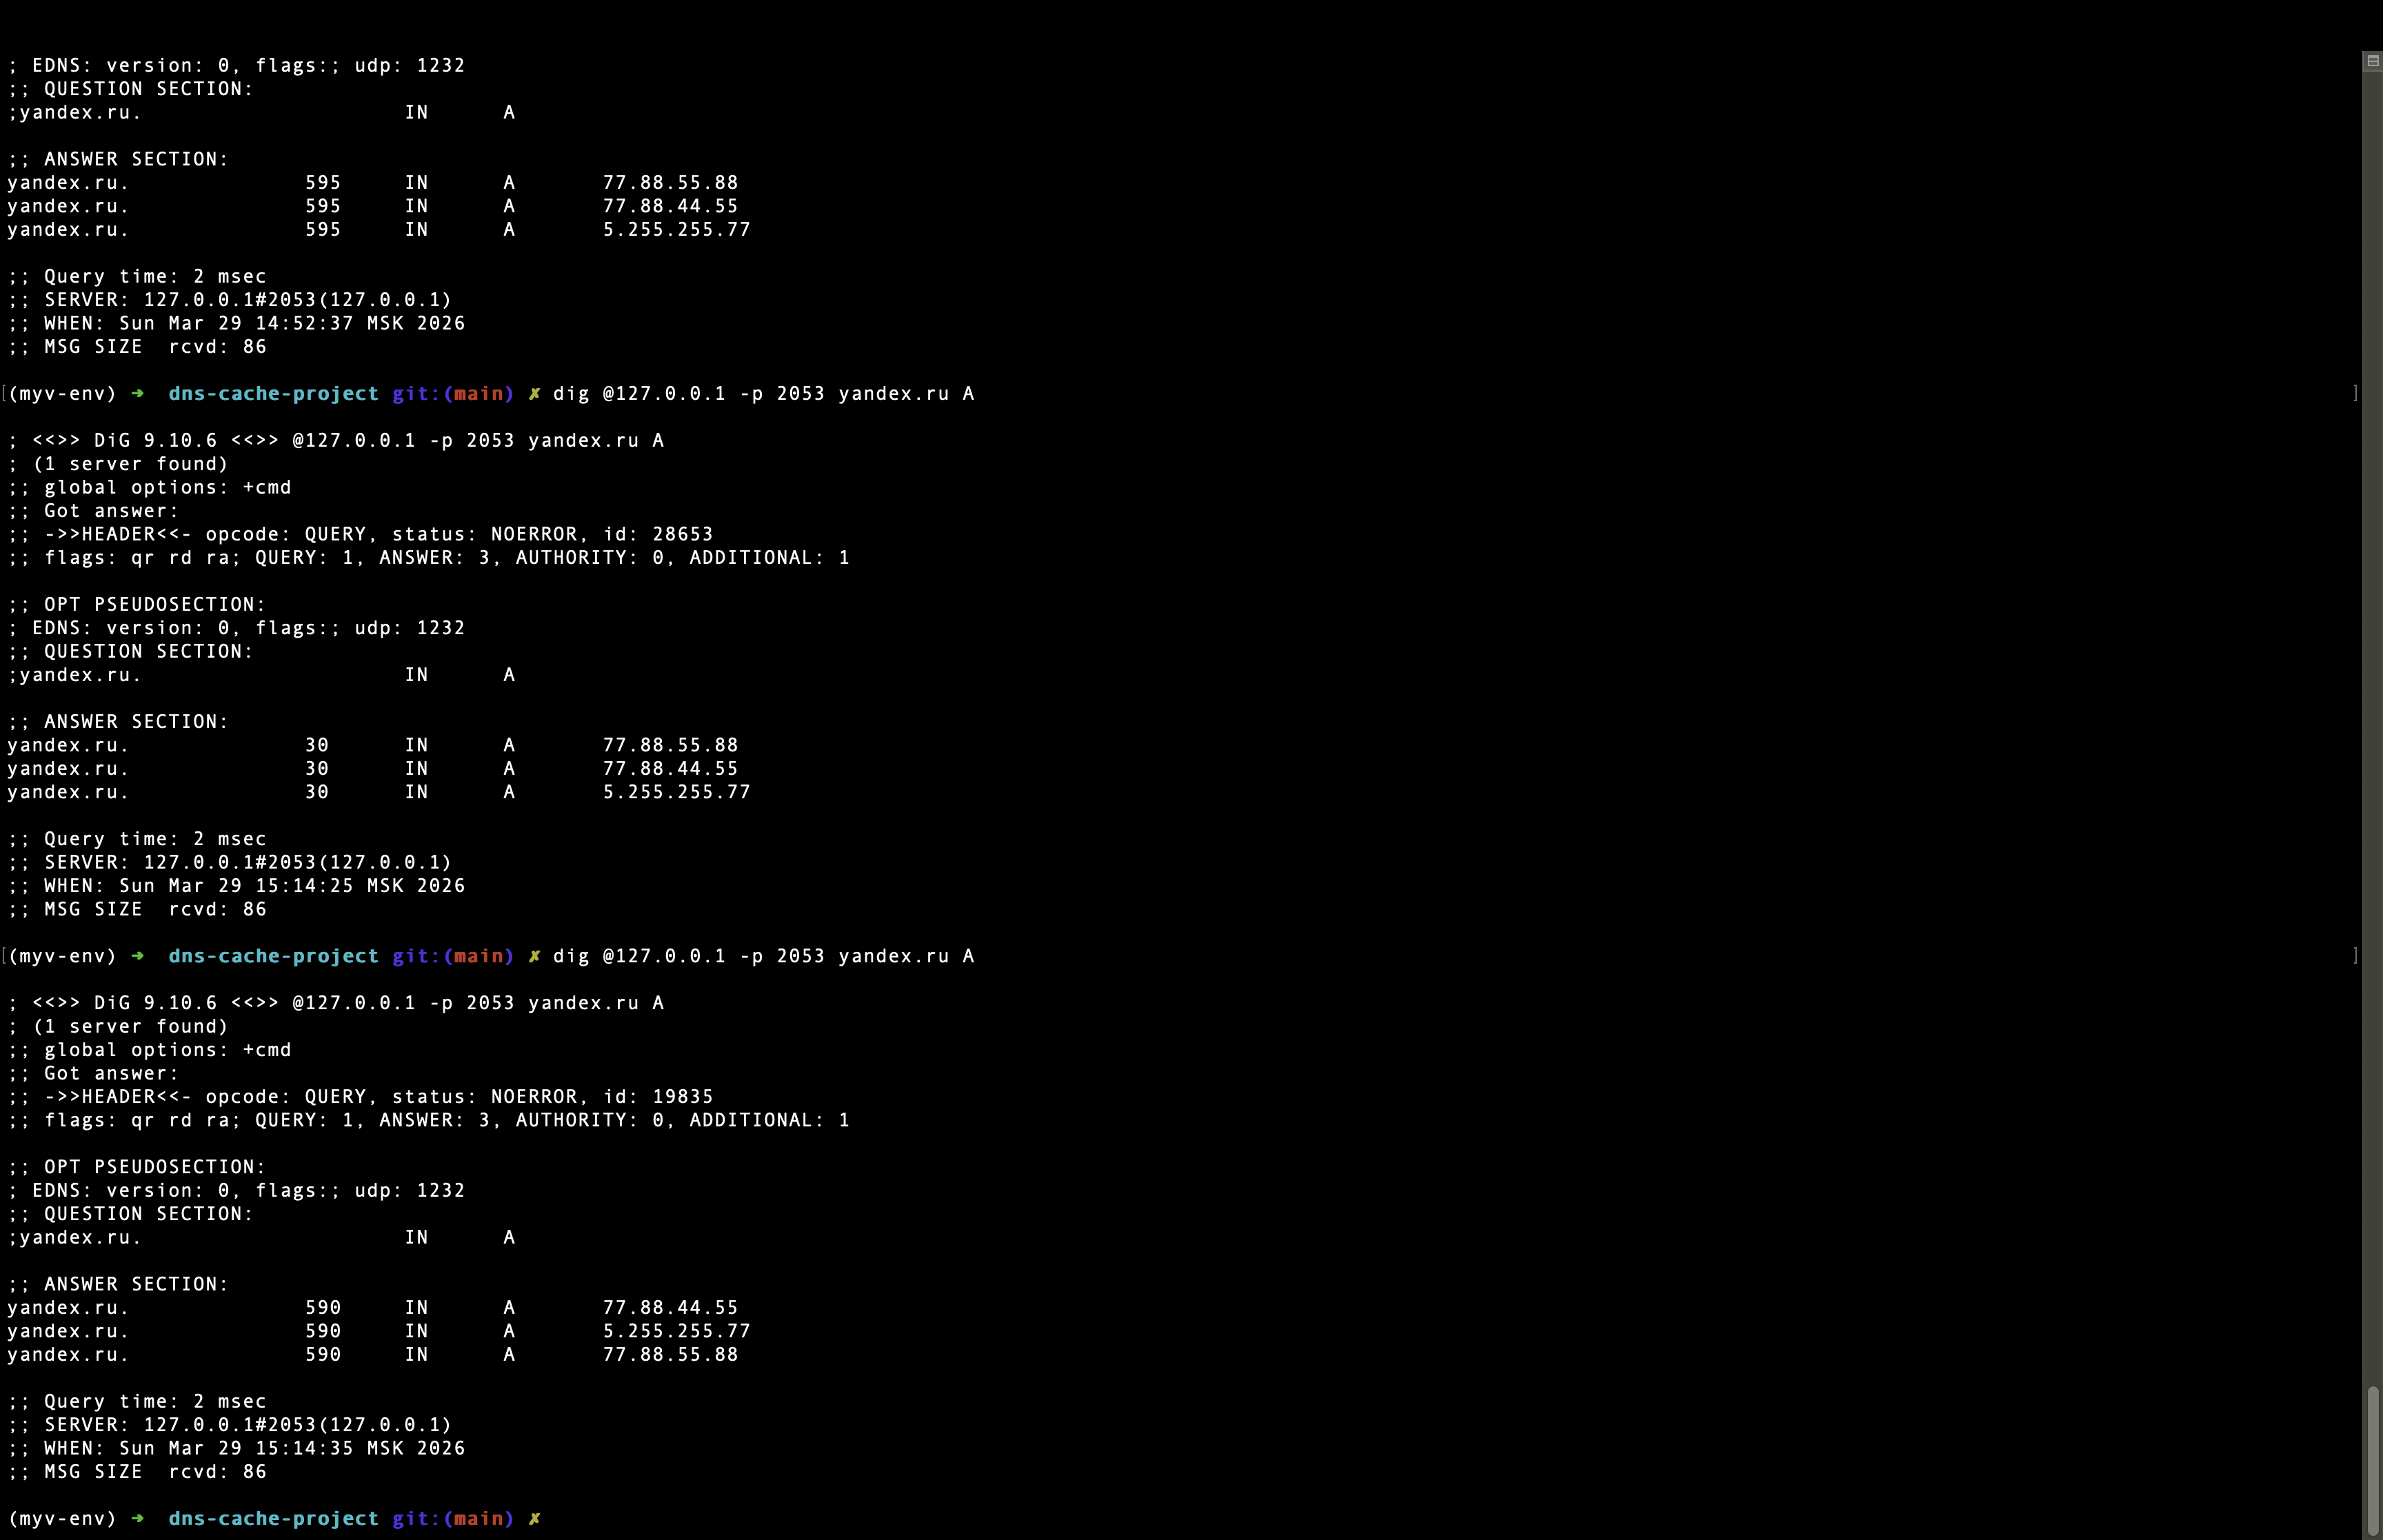
\includegraphics[width=0.95\textwidth]{assets/terminal_screenshot_2.png}
    \caption{Проверка механизма \textit{prefetch} на домене \texttt{yandex.ru}}
\end{figure}

В результате были получены следующие значения:

\begin{lstlisting}
Query time: 2 msec -> Query time: 2 msec

yandex.ru.      30  IN A 77.88.55.88
yandex.ru.      30  IN A 77.88.44.55
yandex.ru.      30  IN A 5.255.255.77

yandex.ru.      590 IN A 77.88.44.55
yandex.ru.      590 IN A 5.255.255.77
yandex.ru.      590 IN A 77.88.55.88
\end{lstlisting}

Важно, что оба ответа были получены практически мгновенно, однако при втором обращении TTL снова стал высоким. Это означает, что запись не была удалена и повторно получена уже после истечения срока хранения, а была обновлена заранее в фоновом режиме.

Дополнительное подтверждение было получено из \texttt{tcpdump}: клиентский ответ возвращался быстро, после чего наблюдались внешние DNS-запросы на обновление записи.

\begin{figure}[H]
    \centering
    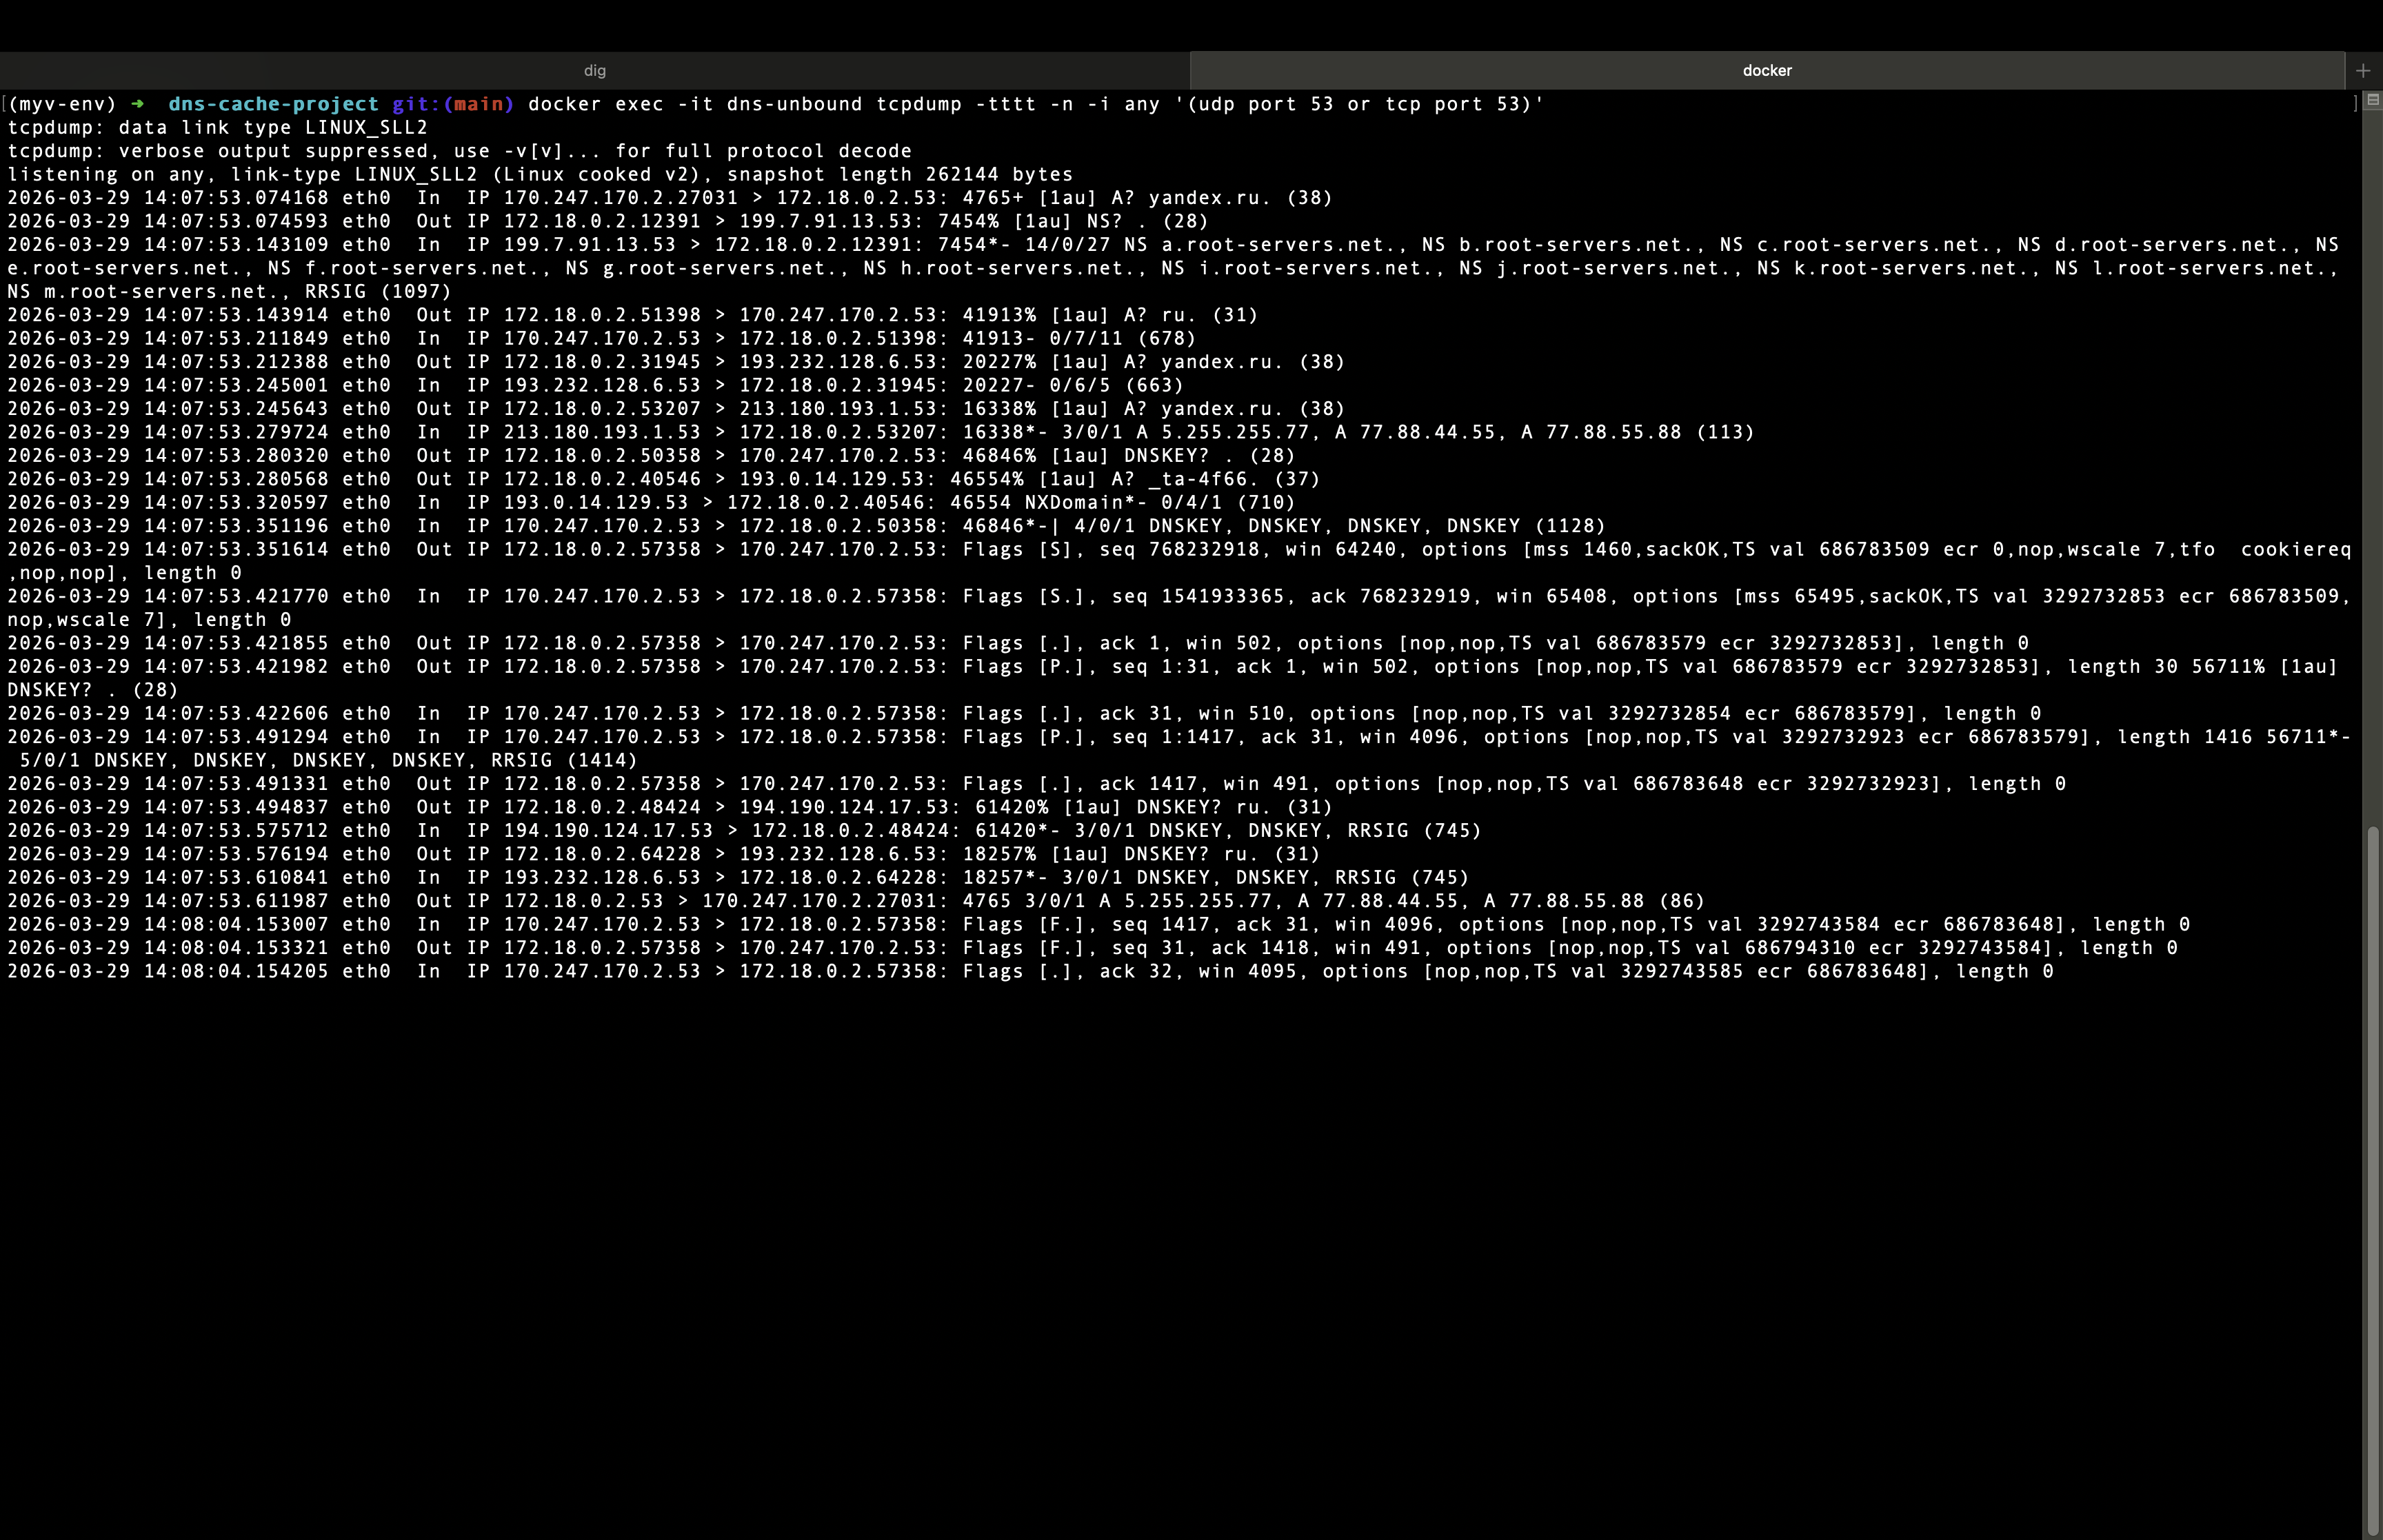
\includegraphics[width=0.9\textwidth]{assets/terminal_screenshot_2_2.png}
    \caption{Сетевой трафик до срабатывания механизма \textit{prefetch}}
\end{figure}

\begin{figure}[H]
    \centering
    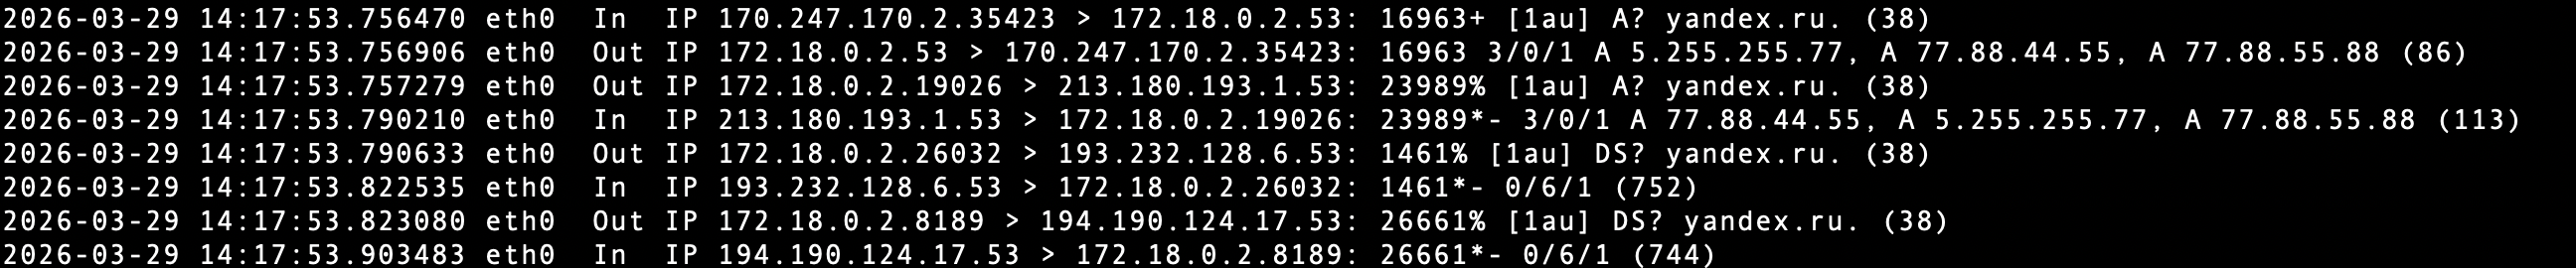
\includegraphics[width=0.9\textwidth]{assets/terminal_screenshot_2_3.png}
    \caption{Сетевой трафик при фоновом обновлении записи механизмом \textit{prefetch}}
\end{figure}

Следовательно, механизм \textit{prefetch} в Unbound успешно работает и позволяет обновлять содержимое кэша до полного истечения TTL без увеличения задержки ответа для клиента.

\subsection{Принудительное изменение времени кэширования средствами Unbound}
В рамках следующего эксперимента проверялась возможность принудительного изменения времени хранения записей стандартными средствами резолвера. Для Unbound такая возможность реализуется, в частности, с помощью параметров \texttt{cache-min-ttl}, \texttt{cache-max-ttl} и \texttt{serve-expired}. В настоящем исследовании основной интерес представлял параметр \texttt{cache-min-ttl}, позволяющий задать минимальное время хранения записи вне зависимости от меньшего значения TTL, полученного от авторитетного сервера.

Для эксперимента был выбран домен \texttt{samokat.ru}, для которого наблюдался TTL порядка 300 секунд. Далее были рассмотрены два режима:
\begin{itemize}
    \item \texttt{cache-min-ttl = 0};
    \item \texttt{cache-min-ttl = 600}.
\end{itemize}

Для чистоты эксперимента параметр \texttt{serve-expired} был отключён. После изменения конфигурации контейнер Unbound пересобирался и перезапускался.

\begin{lstlisting}
docker compose up -d --build unbound
docker compose up -d redis
docker compose ps
\end{lstlisting}

Далее для каждого варианта конфигурации выполнялась одинаковая последовательность действий:

\begin{lstlisting}
dig @127.0.0.1 -p 2053 samokat.ru A
sleep 400
dig @127.0.0.1 -p 2053 samokat.ru A
\end{lstlisting}

При значении \texttt{cache-min-ttl = 0} повторный запрос выполнялся после фактического истечения стандартного TTL, поэтому запись уже отсутствовала во встроенном кэше, и резолвер снова обращался во внешнюю \newline DNS-инфраструктуру.

\begin{figure}[H]
    \centering
    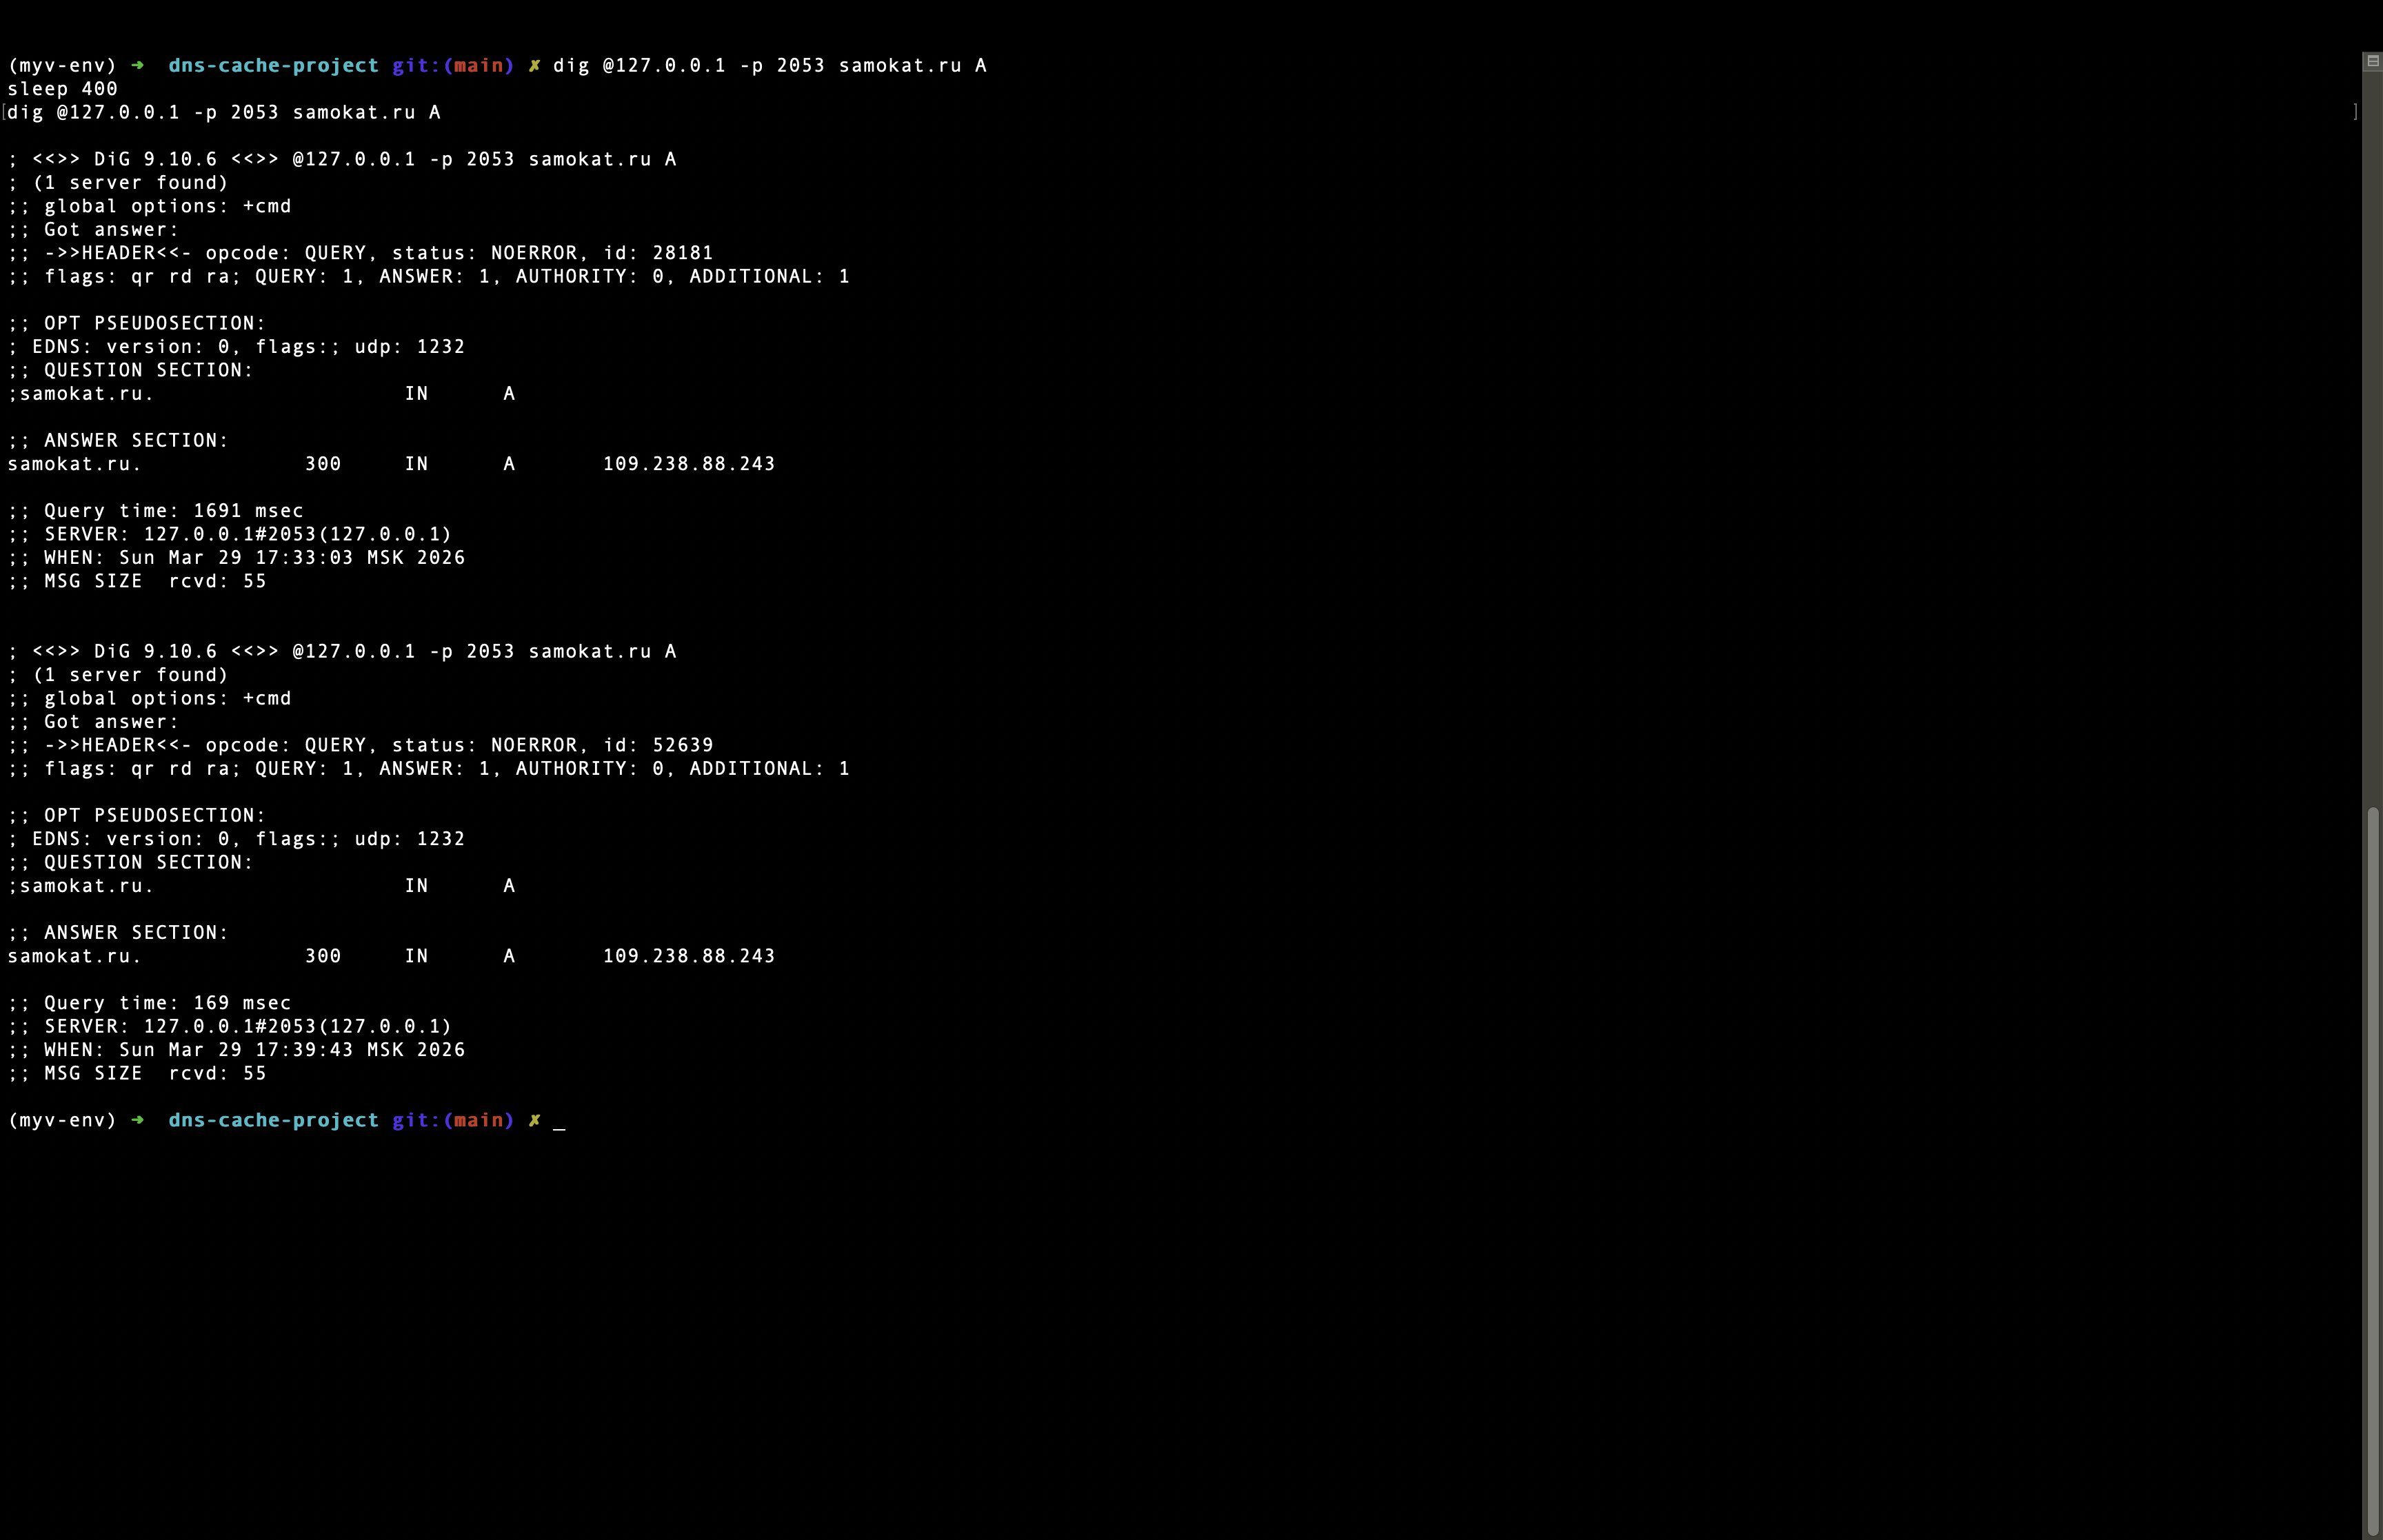
\includegraphics[width=0.95\textwidth]{assets/terminal_screenshot_3.png}
    \caption{Поведение резолвера при \texttt{cache-min-ttl = 0}}
\end{figure}

При значении \texttt{cache-min-ttl = 600} запись сохранялась в кэше дольше исходного TTL, поэтому повторный запрос спустя 400 секунд обслуживался из кэша без нового внешнего обращения.

\begin{figure}[H]
    \centering
    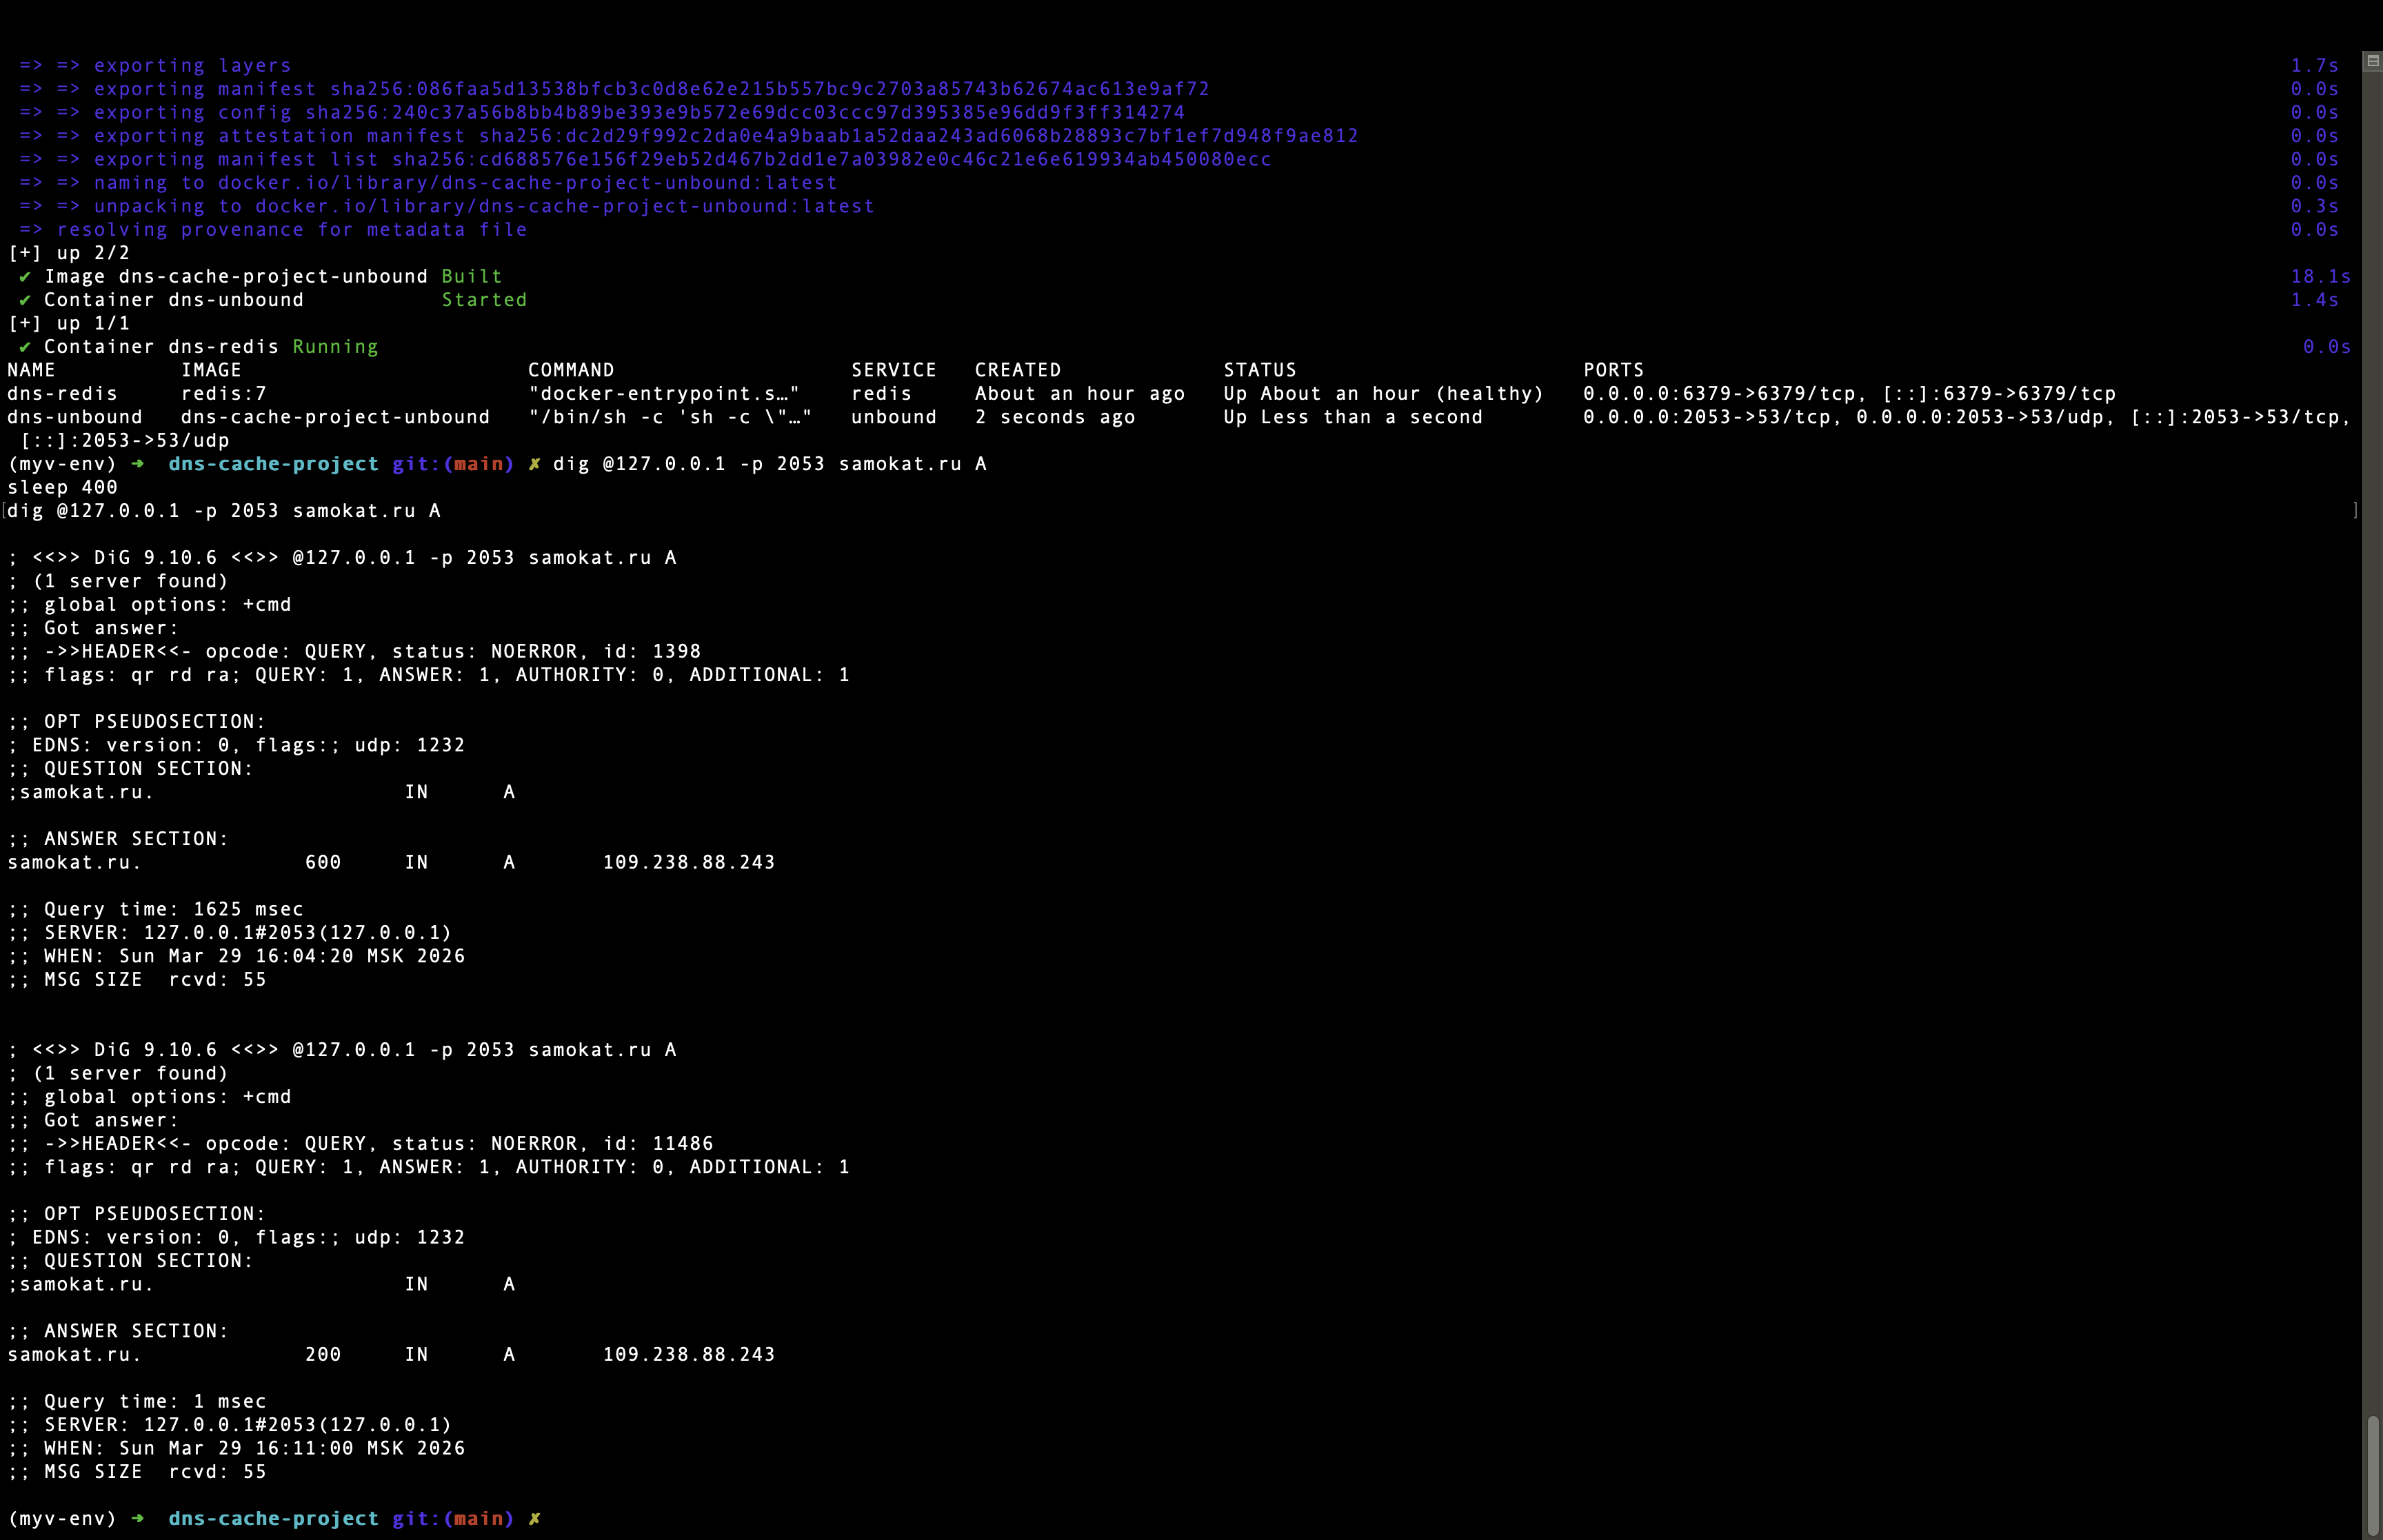
\includegraphics[width=0.95\textwidth]{assets/terminal_screenshot_4.png}
    \caption{Поведение резолвера при \texttt{cache-min-ttl = 600}}
\end{figure}

Сравнение этих двух режимов показывает, что Unbound действительно позволяет административно увеличивать минимальное время хранения кэшируемых записей. Следовательно, средствами самого резолвера возможно реализовать кэширование на время, превышающее исходный TTL, если такая политика допускается выбранной конфигурацией.

\subsection{Проверка вытеснения записей из кэша при ограниченном объёме памяти}
Даже при принудительном увеличении времени хранения встроенный кэш резолвера остаётся ограниченным по объёму. Следовательно, запись может быть удалена не только по истечении TTL, но и вследствие вытеснения из памяти. Целью данного эксперимента было показать, что увеличение \texttt{cache-min-ttl} не гарантирует бессрочного присутствия записи во встроенном кэше при дефиците памяти.

За размеры встроенного кэша в Unbound отвечают параметры:

\begin{lstlisting}
rrset-cache-size: 128m
msg-cache-size: 64m
\end{lstlisting}

Для усиления эффекта вытеснения размеры кэша были искусственно уменьшены, а минимальное время хранения, наоборот, установлено большим. Дополнительно были отключены механизмы \texttt{prefetch} и \texttt{serve-expired}, чтобы не искажать результаты эксперимента.

Временная конфигурация Unbound имела следующий вид:

\begin{lstlisting}
server:
    interface: 0.0.0.0
    port: 53
    access-control: 0.0.0.0/0 allow

    verbosity: 1
    logfile: ""

    directory: "/etc/unbound"
    root-hints: "/etc/unbound/root.hints"
    auto-trust-anchor-file: "/var/lib/unbound/root.key"

    module-config: "validator iterator"

    prefetch: no
    serve-expired: no

    cache-min-ttl: 3600
    cache-max-ttl: 86400

    rrset-cache-size: 256k
    msg-cache-size: 128k

    hide-identity: yes
    hide-version: yes

    do-ip4: yes
    do-ip6: yes
    do-udp: yes
    do-tcp: yes
\end{lstlisting}

После пересборки образа выполнялся контрольный прогрев кэша:

\begin{lstlisting}
docker compose up -d --build unbound
\end{lstlisting}

\begin{lstlisting}
dig @127.0.0.1 -p 2053 yandex.ru A
dig @127.0.0.1 -p 2053 yandex.ru A
\end{lstlisting}

На этом этапе первый запрос требовал внешнего разрешения, а второй уже обслуживался из кэша.

\begin{figure}[H]
    \centering
    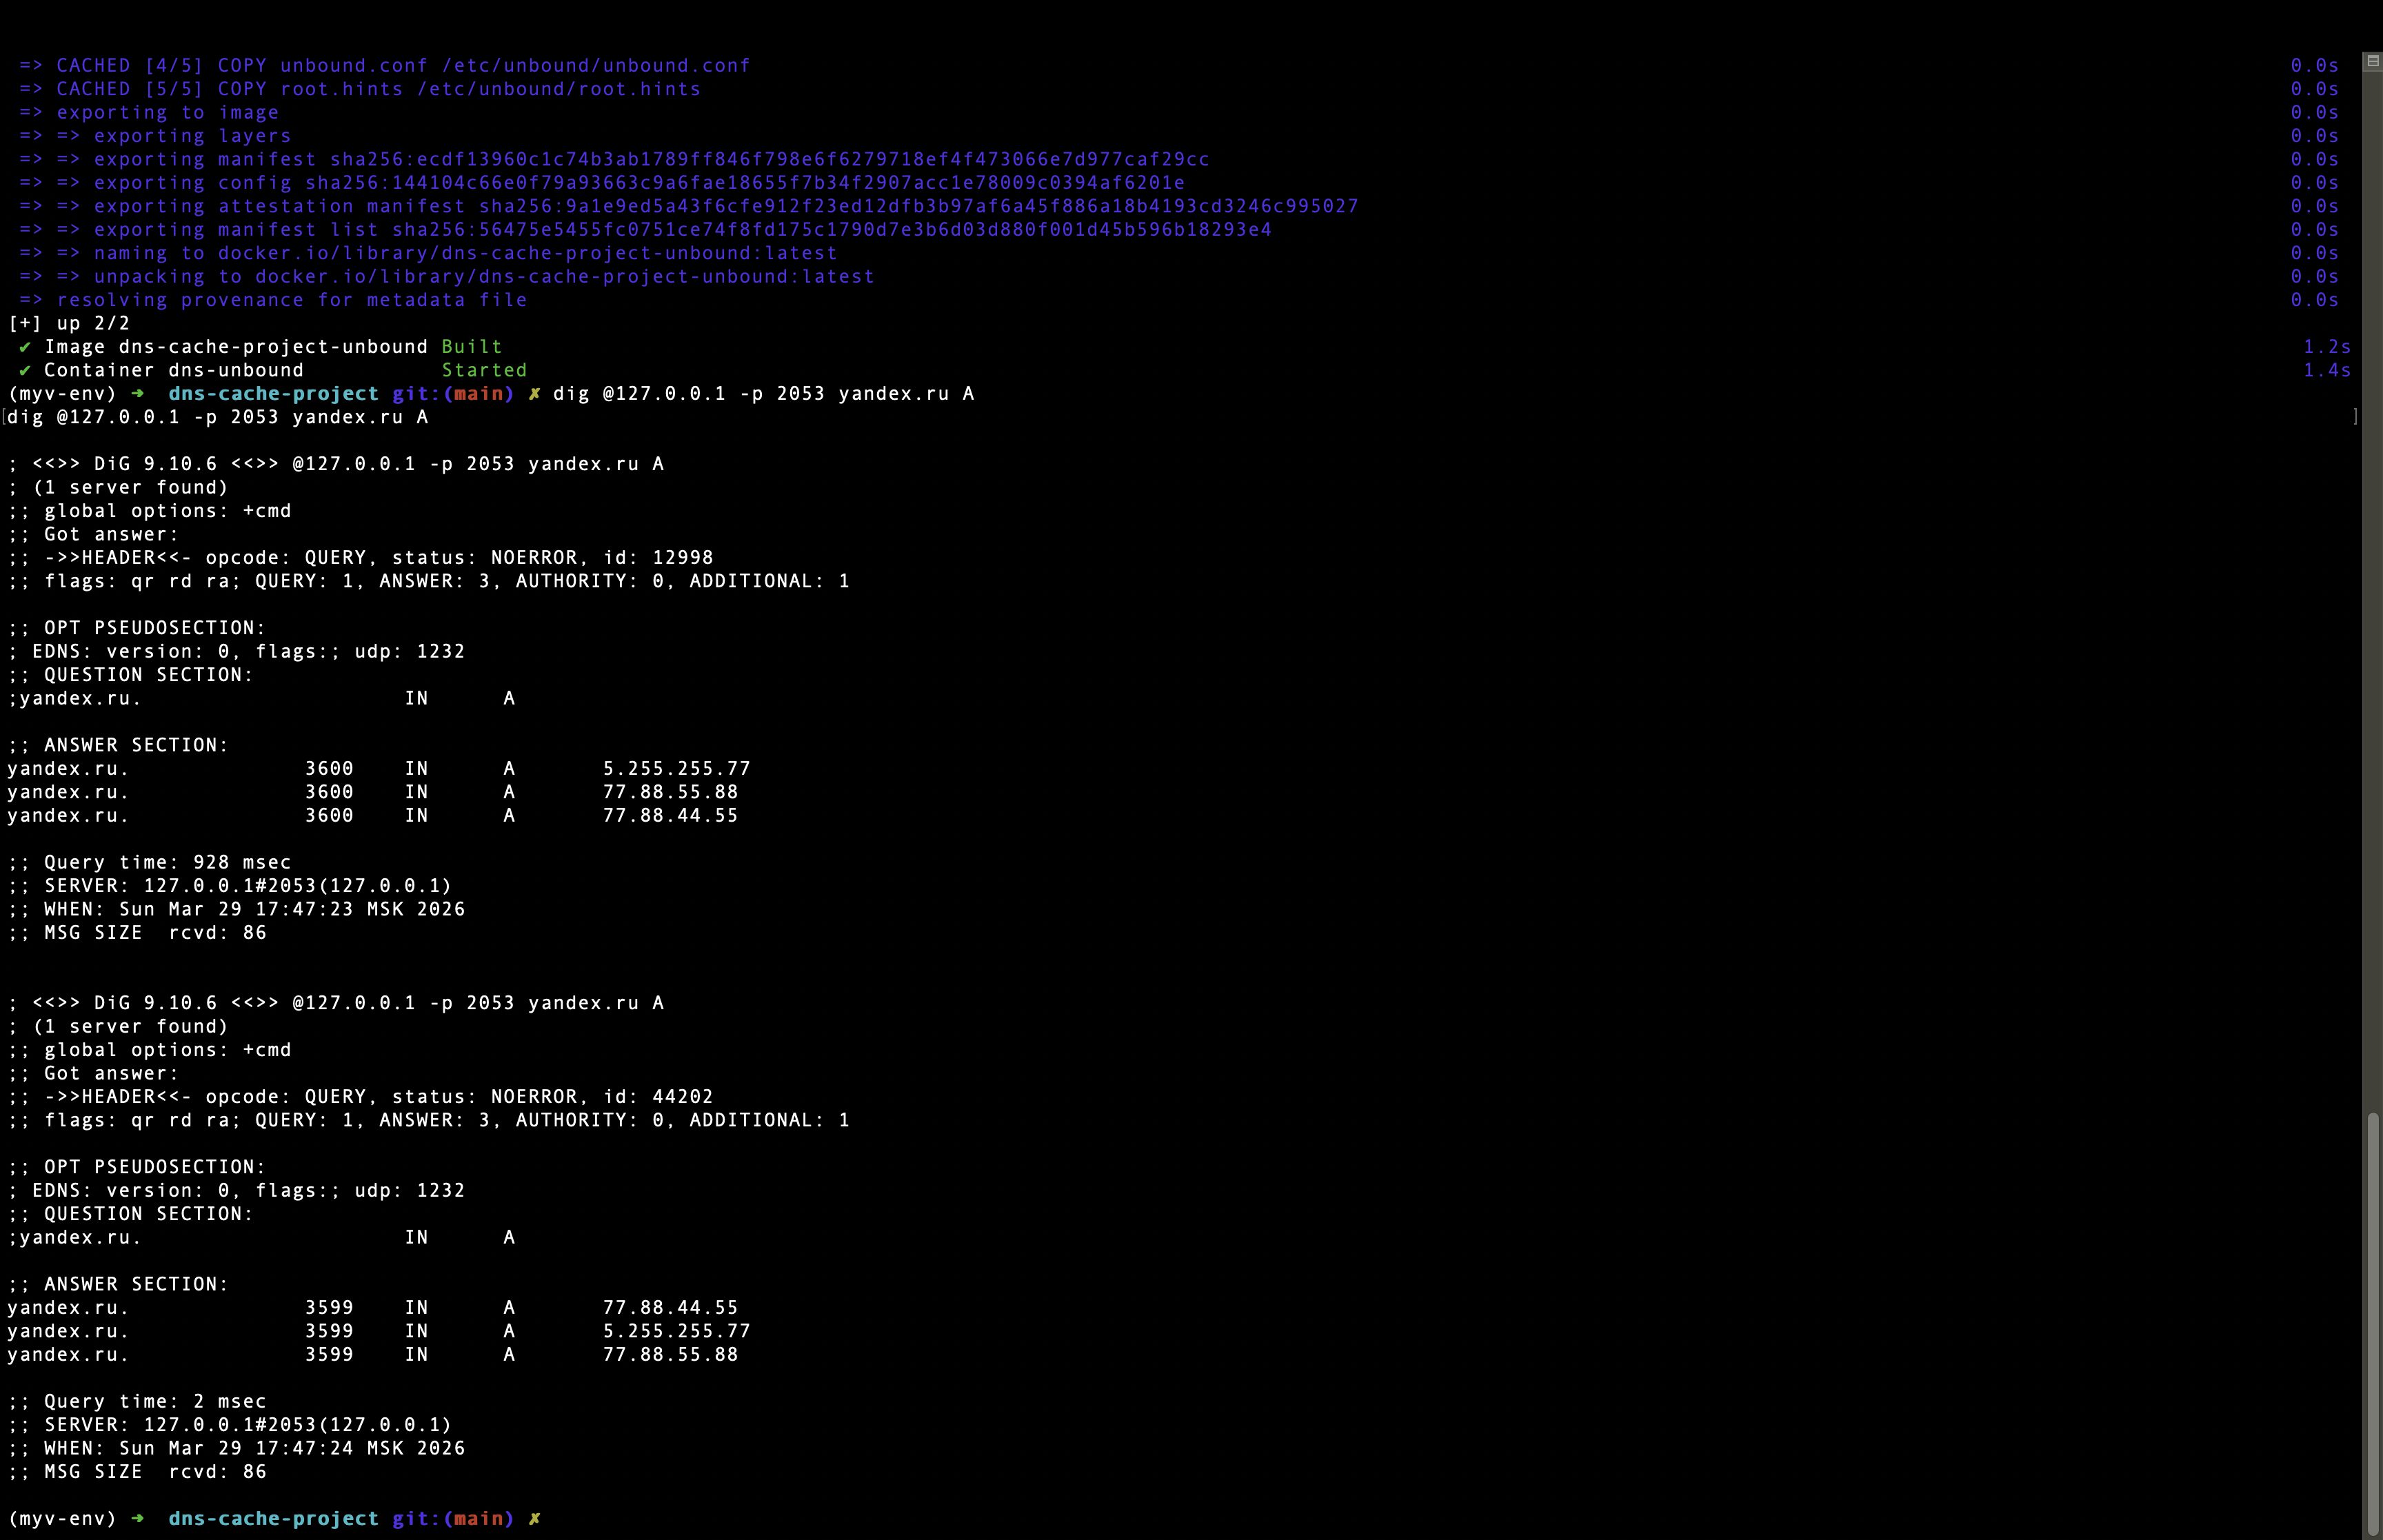
\includegraphics[width=0.95\textwidth]{assets/terminal_screenshot_5_1.png}
    \caption{Контрольное подтверждение работы встроенного кэша перед переполнением}
\end{figure}

Затем кэш нагружался большим количеством уникальных запросов:

\begin{lstlisting}
for i in $(seq 1 1000); do
  dig @127.0.0.1 -p 2053 nx-$i.com A +tries=1 +time=1 > /dev/null 2>&1
  dig @127.0.0.1 -p 2053 nx-$i.com AAAA +tries=1 +time=1 > /dev/null 2>&1
done

dig @127.0.0.1 -p 2053 yandex.ru A
dig @127.0.0.1 -p 2053 yandex.ru A
\end{lstlisting}

\begin{figure}[H]
    \centering
    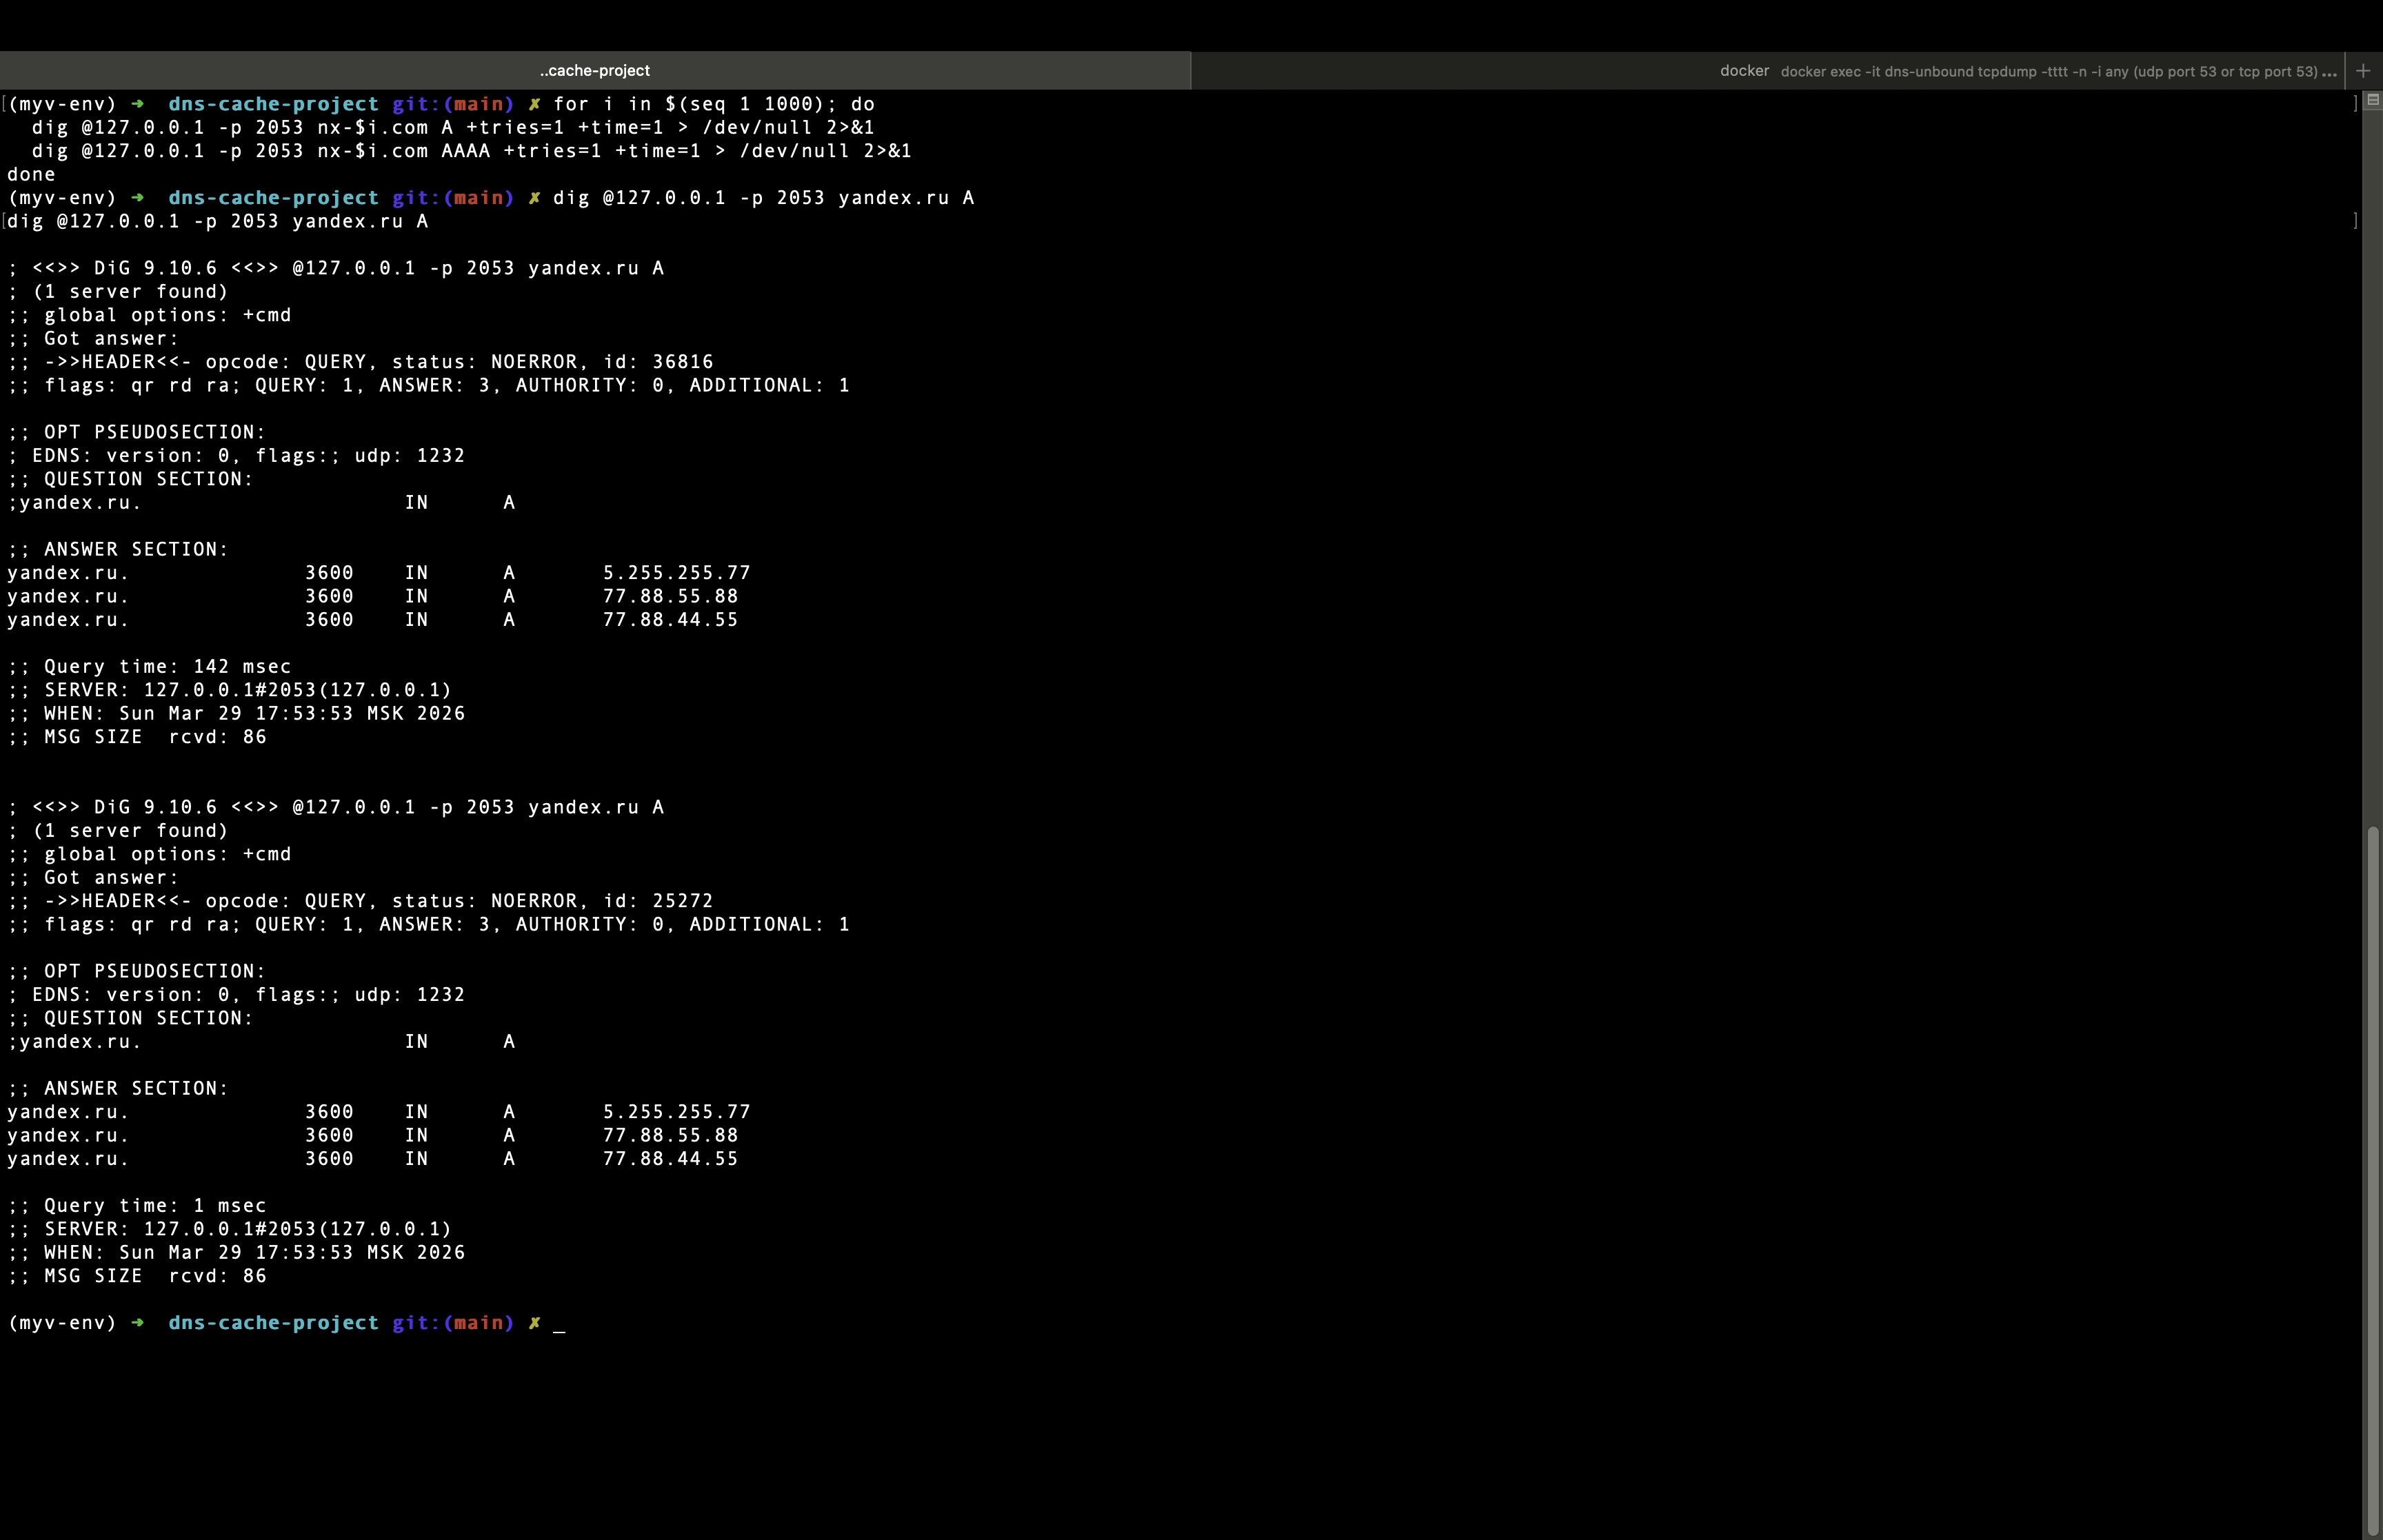
\includegraphics[width=0.95\textwidth]{assets/terminal_screenshot_5_2.png}
    \caption{Поведение резолвера после переполнения встроенного кэша}
\end{figure}

По результатам повторной проверки выяснилось, что запись \texttt{yandex.ru} уже не находилась во встроенном кэше, несмотря на большое значение \newline \texttt{cache-min-ttl}. Первый запрос после нагрузки снова инициировал внешнее DNS-разрешение, а второй запрос уже обслуживался из заново заполненного кэша.

Анализ \texttt{tcpdump} подтвердил этот вывод: сначала резолвер выполнял внешние обращения, затем получал ответ и только после этого возвращал данные клиенту.

\begin{figure}[H]
    \centering
    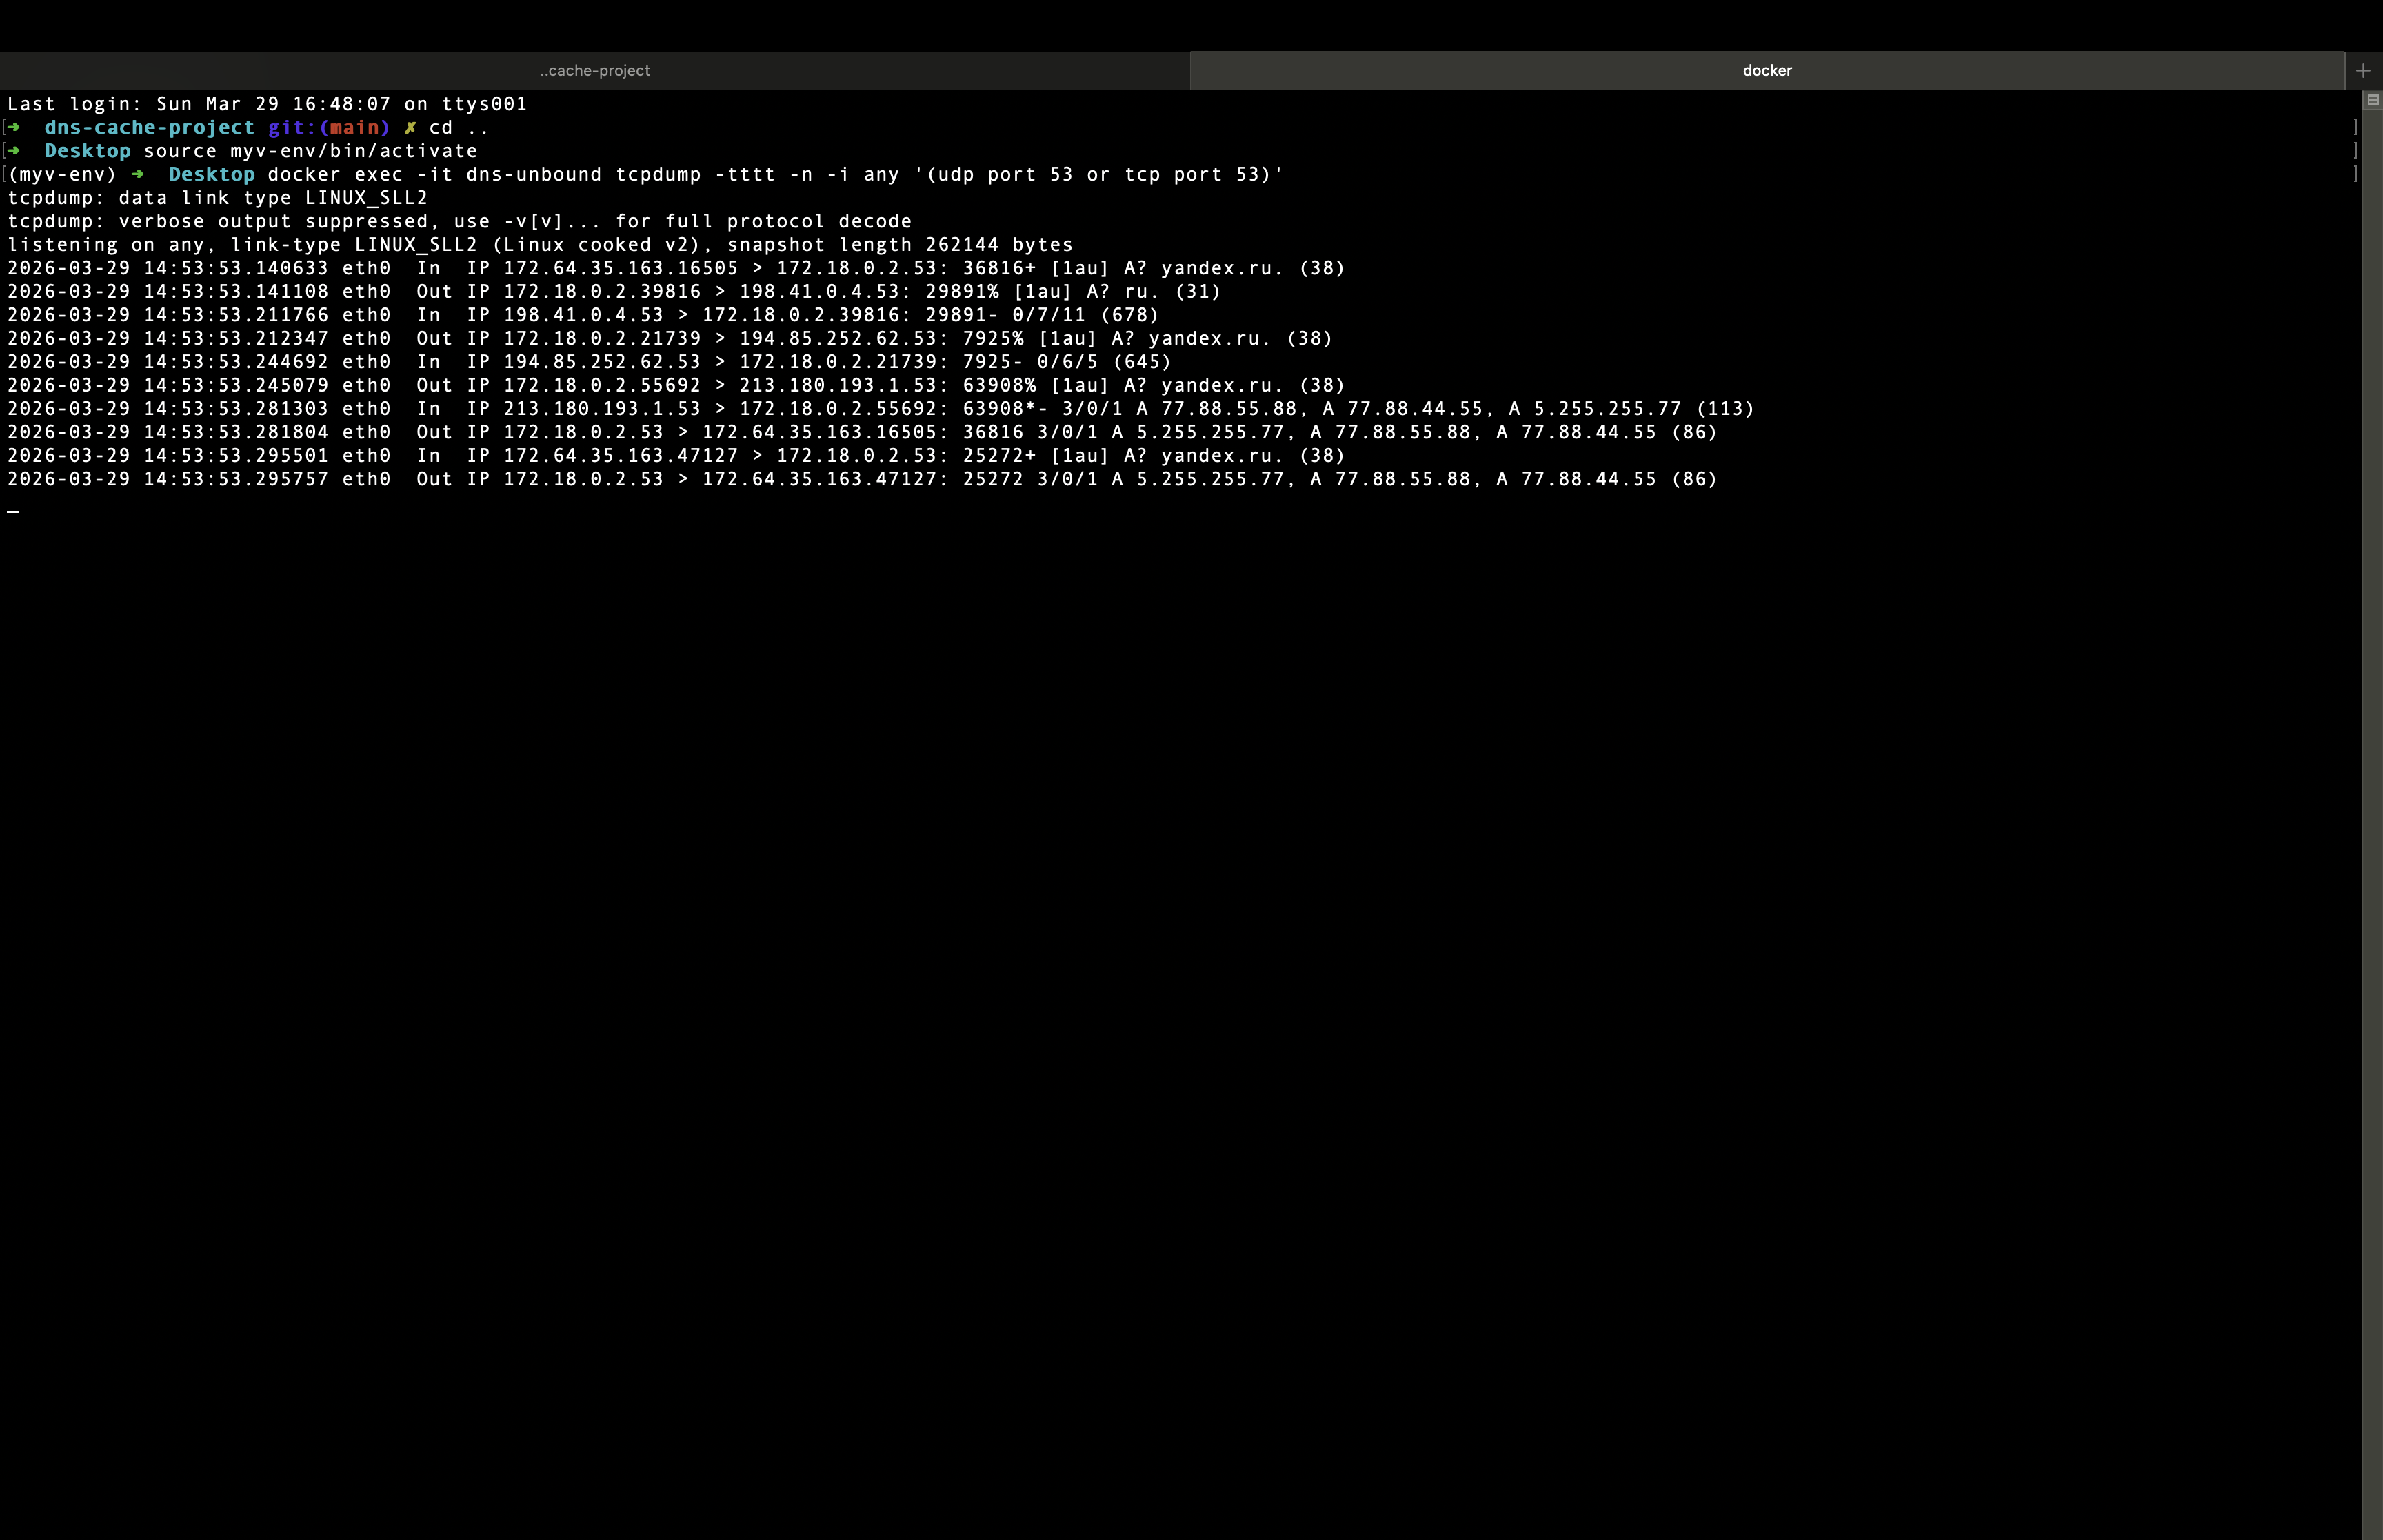
\includegraphics[width=0.95\textwidth]{assets/terminal_screenshot_5_3.png}
    \caption{Сетевое подтверждение вытеснения записи из кэша до истечения TTL}
\end{figure}

Таким образом, было экспериментально показано, что встроенный кэш стандартной сборки резолвера ограничен объёмом памяти. Следовательно, даже при принудительном увеличении времени хранения запись может быть вытеснена раньше и повторно получена из внешней DNS-инфраструктуры.


\section{Реализация внешнего кэша DNS-ответов}

\subsection{Обоснование выбора Redis и PythonMod}

\subsection{Подключение Redis к резолверу}

\subsection{Проверка механизма \texttt{redis\_miss}/\texttt{redis\_hit}}

\subsection{Формирование DNS-ответов из внешней базы данных}

\subsection{Настройка времени хранения ответов, отличного от исходного TTL}

\section{Локальное переопределение DNSSEC-подписанной зоны}

\subsection{Выбор DNSSEC-подписанной зоны}

\subsection{Размещение зоны локально на резолвере}

\subsection{Настройка ответов из локальной зоны}

\subsection{Сбор данных по зоне и генерация локального описания}

\subsection{Подтверждение ответа из локальной базы данных}

\section{Заключение}

Здесь формулируются основные результаты работы и выводы по каждому из этапов исследования.

\section{Список использованных источников}

\begin{enumerate}
    \item Документация Unbound.
    \item Документация Redis.
    \item RFC по DNS, DNSSEC и кэшированию.
    \item Материалы по Docker и сетевой трассировке.
\end{enumerate}

\section*{Приложение А}
\addcontentsline{toc}{section}{Приложение А}

Здесь можно разместить дополнительные листинги конфигурации, скрипты и крупные фрагменты вывода команд.

\section*{Приложение Б}
\addcontentsline{toc}{section}{Приложение Б}

Здесь можно разместить скриншоты и дополнительные иллюстрации.

\end{document}
